% Options for packages loaded elsewhere
\PassOptionsToPackage{unicode}{hyperref}
\PassOptionsToPackage{hyphens}{url}
%
\documentclass[
  english,
  man]{apa6}
\title{DateLife: leveraging databases and analytical tools to reveal the dated Tree of Life}
\author{Luna L. Sánchez Reyes\textsuperscript{1,2}, Emily Jane McTavish\textsuperscript{1}, \& Brian O'Meara\textsuperscript{2}}
\date{}

\usepackage{amsmath,amssymb}
\usepackage{lmodern}
\usepackage{iftex}
\ifPDFTeX
  \usepackage[T1]{fontenc}
  \usepackage[utf8]{inputenc}
  \usepackage{textcomp} % provide euro and other symbols
\else % if luatex or xetex
  \usepackage{unicode-math}
  \defaultfontfeatures{Scale=MatchLowercase}
  \defaultfontfeatures[\rmfamily]{Ligatures=TeX,Scale=1}
\fi
% Use upquote if available, for straight quotes in verbatim environments
\IfFileExists{upquote.sty}{\usepackage{upquote}}{}
\IfFileExists{microtype.sty}{% use microtype if available
  \usepackage[]{microtype}
  \UseMicrotypeSet[protrusion]{basicmath} % disable protrusion for tt fonts
}{}
\makeatletter
\@ifundefined{KOMAClassName}{% if non-KOMA class
  \IfFileExists{parskip.sty}{%
    \usepackage{parskip}
  }{% else
    \setlength{\parindent}{0pt}
    \setlength{\parskip}{6pt plus 2pt minus 1pt}}
}{% if KOMA class
  \KOMAoptions{parskip=half}}
\makeatother
\usepackage{xcolor}
\IfFileExists{xurl.sty}{\usepackage{xurl}}{} % add URL line breaks if available
\IfFileExists{bookmark.sty}{\usepackage{bookmark}}{\usepackage{hyperref}}
\hypersetup{
  pdftitle={DateLife: leveraging databases and analytical tools to reveal the dated Tree of Life},
  pdfauthor={Luna L. Sánchez Reyes1,2, Emily Jane McTavish1, \& Brian O'Meara2},
  pdflang={en-EN},
  pdfkeywords={Tree; Phylogeny; Scaling; Dating; Ages; Divergence times; Open Science; Congruification; Supertree; Calibrations; Secondary calibrations},
  hidelinks,
  pdfcreator={LaTeX via pandoc}}
\urlstyle{same} % disable monospaced font for URLs
\usepackage{graphicx}
\makeatletter
\def\maxwidth{\ifdim\Gin@nat@width>\linewidth\linewidth\else\Gin@nat@width\fi}
\def\maxheight{\ifdim\Gin@nat@height>\textheight\textheight\else\Gin@nat@height\fi}
\makeatother
% Scale images if necessary, so that they will not overflow the page
% margins by default, and it is still possible to overwrite the defaults
% using explicit options in \includegraphics[width, height, ...]{}
\setkeys{Gin}{width=\maxwidth,height=\maxheight,keepaspectratio}
% Set default figure placement to htbp
\makeatletter
\def\fps@figure{htbp}
\makeatother
\setlength{\emergencystretch}{3em} % prevent overfull lines
\providecommand{\tightlist}{%
  \setlength{\itemsep}{0pt}\setlength{\parskip}{0pt}}
\setcounter{secnumdepth}{-\maxdimen} % remove section numbering
% Make \paragraph and \subparagraph free-standing
\ifx\paragraph\undefined\else
  \let\oldparagraph\paragraph
  \renewcommand{\paragraph}[1]{\oldparagraph{#1}\mbox{}}
\fi
\ifx\subparagraph\undefined\else
  \let\oldsubparagraph\subparagraph
  \renewcommand{\subparagraph}[1]{\oldsubparagraph{#1}\mbox{}}
\fi
\newlength{\cslhangindent}
\setlength{\cslhangindent}{1.5em}
\newlength{\csllabelwidth}
\setlength{\csllabelwidth}{3em}
\newlength{\cslentryspacingunit} % times entry-spacing
\setlength{\cslentryspacingunit}{\parskip}
\newenvironment{CSLReferences}[2] % #1 hanging-ident, #2 entry spacing
 {% don't indent paragraphs
  \setlength{\parindent}{0pt}
  % turn on hanging indent if param 1 is 1
  \ifodd #1
  \let\oldpar\par
  \def\par{\hangindent=\cslhangindent\oldpar}
  \fi
  % set entry spacing
  \setlength{\parskip}{#2\cslentryspacingunit}
 }%
 {}
\usepackage{calc}
\newcommand{\CSLBlock}[1]{#1\hfill\break}
\newcommand{\CSLLeftMargin}[1]{\parbox[t]{\csllabelwidth}{#1}}
\newcommand{\CSLRightInline}[1]{\parbox[t]{\linewidth - \csllabelwidth}{#1}\break}
\newcommand{\CSLIndent}[1]{\hspace{\cslhangindent}#1}
\DeclareUnicodeCharacter{0301}{*************************************}
% Manuscript styling
\usepackage{upgreek}
\captionsetup{font=singlespacing,justification=justified}

% Table formatting
\usepackage{longtable}
\usepackage{lscape}
% \usepackage[counterclockwise]{rotating}   % Landscape page setup for large tables
\usepackage{multirow}		% Table styling
\usepackage{tabularx}		% Control Column width
\usepackage[flushleft]{threeparttable}	% Allows for three part tables with a specified notes section
\usepackage{threeparttablex}            % Lets threeparttable work with longtable

% Create new environments so endfloat can handle them
% \newenvironment{ltable}
%   {\begin{landscape}\centering\begin{threeparttable}}
%   {\end{threeparttable}\end{landscape}}
\newenvironment{lltable}{\begin{landscape}\centering\begin{ThreePartTable}}{\end{ThreePartTable}\end{landscape}}

% Enables adjusting longtable caption width to table width
% Solution found at http://golatex.de/longtable-mit-caption-so-breit-wie-die-tabelle-t15767.html
\makeatletter
\newcommand\LastLTentrywidth{1em}
\newlength\longtablewidth
\setlength{\longtablewidth}{1in}
\newcommand{\getlongtablewidth}{\begingroup \ifcsname LT@\roman{LT@tables}\endcsname \global\longtablewidth=0pt \renewcommand{\LT@entry}[2]{\global\advance\longtablewidth by ##2\relax\gdef\LastLTentrywidth{##2}}\@nameuse{LT@\roman{LT@tables}} \fi \endgroup}

% \setlength{\parindent}{0.5in}
% \setlength{\parskip}{0pt plus 0pt minus 0pt}

% Overwrite redefinition of paragraph and subparagraph by the default LaTeX template
% See https://github.com/crsh/papaja/issues/292
\makeatletter
\renewcommand{\paragraph}{\@startsection{paragraph}{4}{\parindent}%
  {0\baselineskip \@plus 0.2ex \@minus 0.2ex}%
  {-1em}%
  {\normalfont\normalsize\bfseries\itshape\typesectitle}}

\renewcommand{\subparagraph}[1]{\@startsection{subparagraph}{5}{1em}%
  {0\baselineskip \@plus 0.2ex \@minus 0.2ex}%
  {-\z@\relax}%
  {\normalfont\normalsize\itshape\hspace{\parindent}{#1}\textit{\addperi}}{\relax}}
\makeatother

% \usepackage{etoolbox}
\makeatletter
\patchcmd{\HyOrg@maketitle}
  {\section{\normalfont\normalsize\abstractname}}
  {\section*{\normalfont\normalsize\abstractname}}
  {}{\typeout{Failed to patch abstract.}}
\patchcmd{\HyOrg@maketitle}
  {\section{\protect\normalfont{\@title}}}
  {\section*{\protect\normalfont{\@title}}}
  {}{\typeout{Failed to patch title.}}
\makeatother

\usepackage{xpatch}
\makeatletter
\xapptocmd\appendix
  {\xapptocmd\section
    {\addcontentsline{toc}{section}{\appendixname\ifoneappendix\else~\theappendix\fi\\: #1}}
    {}{\InnerPatchFailed}%
  }
{}{\PatchFailed}
\keywords{Tree; Phylogeny; Scaling; Dating; Ages; Divergence times; Open Science; Congruification; Supertree; Calibrations; Secondary calibrations\newline\indent Word count: 4586}
\DeclareDelayedFloatFlavor{ThreePartTable}{table}
\DeclareDelayedFloatFlavor{lltable}{table}
\DeclareDelayedFloatFlavor*{longtable}{table}
\makeatletter
\renewcommand{\efloat@iwrite}[1]{\immediate\expandafter\protected@write\csname efloat@post#1\endcsname{}}
\makeatother
\usepackage{lineno}

\linenumbers
\usepackage{csquotes}
\ifXeTeX
  % Load polyglossia as late as possible: uses bidi with RTL langages (e.g. Hebrew, Arabic)
  \usepackage{polyglossia}
  \setmainlanguage[]{english}
\else
  \usepackage[main=english]{babel}
% get rid of language-specific shorthands (see #6817):
\let\LanguageShortHands\languageshorthands
\def\languageshorthands#1{}
\fi
\ifLuaTeX
  \usepackage{selnolig}  % disable illegal ligatures
\fi


\shorttitle{DateLife: revealing the dated Tree of Life}

\authornote{

School of Natural Sciences, University of California, Merced, Science and Engineering Building 1.

Department of Ecology and Evolutionary Biology, University of Tennessee, Knoxville, 446 Hesler Biology Building, Knoxville, TN 37996, USA.

The authors made the following contributions. Luna L. Sánchez Reyes: Data curation, Investigation, Software, Visualization, Validation, Writing - Original Draft Preparation, Writing - Review \& Editing; Emily Jane McTavish: Resources, Software, Writing - Review \& Editing; Brian O'Meara: Conceptualization, Funding acquisition, Methodology, Resources, Software, Supervision, Writing - Review \& Editing.

Correspondence concerning this article should be addressed to Luna L. Sánchez Reyes, . E-mail: \href{mailto:sanchez.reyes.luna@gmail.com}{\nolinkurl{sanchez.reyes.luna@gmail.com}}

}

\affiliation{\vspace{0.5cm}\textsuperscript{1} University of California, Merced\\\textsuperscript{2} University of Tennessee, Knoxville}

\abstract{%
Date estimates for times of evolutionary divergences are key data for research in the natural sciences. These estimates also provide valuable information for for education, science communication, and policy decisions.
Although achieving a high-quality reconstruction of a phylogenetic tree with branch lengths proportional to absolute time (chronogram) is a difficult and time-consuming task, the increased availability of fossil and molecular data, and time-efficient analytical techniques has resulted in many recent publications of large chronograms for a large number and wide diversity of organisms.
When these estimates are shared in public, open databases this wealth of expertly-curated and peer-reviewed data on time of evolutionary origin is exposed in a programatic and reusable way.
Intensive and localized efforts have improved data sharing practices, as well as incentivizited open science in biology.
Here we present DateLife, a service implemented as an R package and an R Shiny website application available at www.datelife.org, that provides functionalities for efficient and easy finding, summary, reuse, and reanalysis of expert, peer-reviewed, public data on time of evolutionary origin.
The main DateLife workflow constructs a chronogram for any given combination of taxon names by searching a local chronogram database constructed and curated from the Open Tree of Life Phylesystem phylogenetic database, which incorporates phylogenetic data from the TreeBASE database as well.
We implement and test methods for summarizing time data from multiple source chronograms using supertree and congruification algorithms, and using age data extracted from source chronograms as secondary calibration points to add branch lengths proportional to absolute time to a tree topology.
DateLife will be useful to increase awereness of the existing variation in expert time of divergence data, and can foster exploration of the effect of alternative divergence time hypotheses on the results of analyses, providing a framework for a more informed interpretation of evolutionary results.
}



\begin{document}
\maketitle

\hypertarget{introduction}{%
\section{Introduction}\label{introduction}}

Chronograms --phylogenies with branch lengths proportional to time-- provide key data for the study of natural processes in many areas of biological research, such as developmental biology (Delsuc et al., 2018; Laubichler \& Maienschein, 2009), conservation biology (Felsenstein, 1985; C. Webb, 2000), historical biogeography (Posadas, Crisci, \& Katinas, 2006), and species diversification (Magallon \& Sanderson, 2001; Morlon, 2014).

Building a chronogram is not an easy task.
It requires obtaining and curating data to construct a phylogeny, selecting and placing appropriate calibrations on the phylogeny using independent age data points from the fossil record or other dated events, and inferring the full dated tree;
it also generally requires specialized biological training, taxonomic domain knowledge, and a non-negligible amount of research time, computational resources and funding.

Here we present the DateLife project which has the main goal of capturing data from published chronograms, and making these data readily accessible to users for reuse and reanalysis.
DateLife's core software application is available as an R package (Sanchez-Reyes et al., 2022), and as an online Rshiny interactive website at www.datelife.org. It features key elements for scientific reproducibility, such as a versioned, open and fully public source database (McTavish et al., 2015), data stored and available in a computer readable format (Vos et al., 2012), automated and programmatic ways of accessing the data (Stoltzfus et al., 2013) and methods to summarize and compare the data.

\hypertarget{description}{%
\section{Description}\label{description}}

DateLife's core software application consists of the R package \texttt{datelife}. Its latest stable version -- v0.6.2, is available from the CRAN repository (Sanchez-Reyes et al., 2022), and relies on functionalities from various biological R packages:
ape (Paradis, Claude, \& Strimmer, 2004),
bold (Chamberlain et al., 2019),
geiger (Pennell et al., 2014),
paleotree (Bapst, 2012),
phyloch (Heibl, 2008),
phylocomr (Ooms \& Chamberlain, 2018),
phytools (Revell, 2012),
rotl (Michonneau, Brown, \& Winter, 2016), and
taxize (Chamberlain \& Szöcs, 2013; Chamberlain et al., 2019).
Figure \ref{fig:workflow} provides a graphical summary of the three main steps of the DateLife algorithm: creating a search query, searching a database, and summarizing results from the search.

\hypertarget{creating-a-search-query}{%
\subsection{Creating a search query}\label{creating-a-search-query}}

DateLife starts by processing an input consisting of at least two taxon names, which can be provided as a comma separated character string or as tip labels on a tree. If the input is a tree, it can be provided as a classic newick character string (Archie et al., 1986), or as a ``phylo'' R object (Paradis et al., 2004). The input tree is not required to have branch lengths, and its topology is used in the summary steps described below.

DateLife accepts scientific names that can belong to any inclusive taxonomic group (e.g., genus, family, tribe, etc.) or a binomial species name. Subspecies and variants are ignored. If an input taxon name belongs to an inclusive taxonomic group the algorithm has two alternative behaviors defined by the ``get species from taxon'' flag. If the flag is active, DateLife retrieves all species names within the inclusive taxonomic group (according to a taxonomy) and adds them to the input string. If the flag is inactive, DateLife excludes the taxon names above the species level from the input.

DateLife processes input scientific names using a Taxonomic Name Resolution Service (TNRS), which increases the probability of correctly finding the queried taxon names in the chronogram database. TNRS detects, corrects and standardizes name misspellings and typos, variant spellings and authorities, and nomenclatural synonyms to a single taxonomic standard (Boyle et al., 2013). DateLife implements TNRS using OpenTree's unified taxonomy as standard (Open Tree Of Life et al., 2016; Rees \& Cranston, 2017), storing OpenTree's Taxonomy identification numbers for further processing.

The processed input taxon names are saved as an R object of a newly defined class \texttt{datelifeQuery} that is used in the following steps. This object contains the standardized names, the corresponding OpenTree taxonomic id numbers, and the topology of the input tree if any was provided.

\hypertarget{searching-a-chronogram-database}{%
\subsection{Searching a chronogram database}\label{searching-a-chronogram-database}}

DateLife's chronogram database latest version consist of 253 chronograms published in 187 different studies. It is curated from OpenTree's phylogenetic database, the Phylesystem, which constitutes an open source of expert and peer-reviewed phylogenetic knowledge with rich metadata (McTavish et al., 2015), which allows automatic and reproducible assembly of our chronogram database. Datelife's chronogram database is navigable as an R data object within the \texttt{datelife} R package.
Published chronograms can be added to Phylesystem by any user, at any time, and are immediately publicly available (\url{https://tree.opentreeoflife.org/curator}). A user may then update their local cache of DateLife's chronogram database to include new chronogram data on a following search.

A DateLife search is implemented by matching processed taxon names provided by the user to tip labels in the chronogram database. Chronograms with at least two matching taxon names on their tip labels are identified and pruned down to preserve only the matched taxa.
These matching pruned chronograms are referred to as source chronograms.
Total distance (in units of millions of years) between taxon pairs within each source chronogram are stored as a patristic distance matrix (Figure \ref{fig:workflow}).
The matrix format speeds up extraction of pairwise taxon ages of any queried taxa, as opposed to searching the ancestor node of a pair of taxa in a ``phylo'' object or newick string.
Finally, the patristic matrices are associated to the study citation where the original chronogram was published, and stored as an R object of the newly defined class \texttt{datelifeResult}.

\hypertarget{summarizing-search-results}{%
\subsection{Summarizing search results}\label{summarizing-search-results}}

Summary information is extracted from the \texttt{datelifeResult} object to inform decisions for subsequent steps in the analysis workflow. Basic summary information available to the user is:

\begin{enumerate}
\def\labelenumi{\arabic{enumi}.}
\tightlist
\item
  The matching pruned chronograms as newick strings or ``phylo'' objects.
\item
  The ages of the root of all source chronograms. These ages can correspond to the age of the most recent common ancestor (mrca) of the user's group of interest if the source chronograms have all taxa belonging to the group. If not, the root corresponds to the mrca of a subgroup withing the group of interest.
\item
  Study citations where original chronograms were published.
\item
  A report of input taxon names matches across source chronograms.
\item
  The source chronogram(s) with the most input taxon names.
\item
  Various single summary chronograms resulting from summarizing age data, generated using the methodology described below.
\end{enumerate}

\emph{\textbf{Choosing a topology.--}}
DateLife requires a tree topology to summarize age data upon.
We recommend that users provide a tree topology as input from the literature, or one of their own making. If no topology is provided, DateLife automatically subsets one from the OpenTree synthetic tree (Open Tree Of Life et al., 2019).
Alternatively, DateLife can combine topologies from source chronograms using a supertree approach.
To combine topologies from source chronograms into a single summary (or supertree) topology, the DateLife algorithm starts by identifying the source chronograms that form a grove, roughly, a sufficiently overlapping set of taxa between trees, by implementing definition 2.8 for n-overlap from Ané et al. (2009). In rare cases, a group of trees can have multiple groves. By default, DateLife chooses the grove with the most taxa, however, the ``criterion = trees'' flag allows the user to choose the grove with the most trees instead.
If source chronograms do not form a grove, the supertree reconstruction will fail.

\emph{\textbf{Dating the topology.--}}
Input topologies from OpenTree or the supertree approach described above do not include branch length estimates of any kind.
Optionally, to estimate branch lengths proportional to substitution rates on these topologies, DateLife can mine the Barcode of Life Data System, BOLD (Ratnasingham \& Hebert, 2007) to obtain genetic markers for the input taxa.
These markers are aligned with MUSCLE (Edgar, 2004) (by default) or MAFFT (Katoh, Asimenos, \& Toh, 2009).
This alignment can be used to estimate branch lengths on input topologies that lack branch lengths.
Currently, branch length reconstruction in DateLife is performed using parsimony and the likelihood of the phylogenetic tree given a sequence alignment is computed (Schliep, 2011).
While relative branch length information provides additional data for nodes without secondary date calibrations, topologies without branch lengths can also be dated.

Once a topology is chosen, DateLife applies the congruification method (Eastman, Harmon, \& Tank, 2013) to find nodes belonging to the same clade across source chronograms, and extract the corresponding node ages from the patristic distance matrices stored as \texttt{datelifeResult}. By definition, the matrices store total distance (time from tip to tip), hence, node ages correspond to half the values stored in the patristic distance matrices.
This assumes that the terminal taxa are coeval and occur at the present.
A table of congruified node ages that can be used as secondary calibrations is stored as a \texttt{congruifiedCalibrations} object.

For each congruent node, the pairwise distances that traverse that node are summarized into a single summary matrix using classic summary statistics (i.e., mean, median, minimum and maximum ages), and the Supermatrix Distance Method {[}SDM; Criscuolo, Berry, Douzery, and Gascuel (2006){]}, which deforms patristic distance matrices by minimizing variance and then averaging them.
These single summary taxon pair age matrices (Summarized calibrations) can be applied as secondary calibrations to date a tree topology, using different dating methods currently supported within DateLife: MrBayes (Huelsenbeck \& Ronquist, 2001; Ronquist \& Huelsenbeck, 2003), PATHd8 (Britton, Anderson, Jacquet, Lundqvist, \& Bremer, 2007), BLADJ (Campbell O. Webb, Ackerly, \& Kembel, 2008; Campbell O. Webb \& Donoghue, 2005), and treePL (Stephen A. Smith \& O'Meara, 2012).

By default, DateLife implements the Branch Length Adjuster (BLADJ) algorithm to obtain a fully dated topology. BLADJ fixes node ages that have calibration data, and distributes time between nodes with no data evenly between nodes with calibration data.
This minimizes age variance in the resulting chronogram (Campbell O. Webb et al., 2008).
BLADJ does not incorporate input phylogeny branch lengths even when they are present.
When there is conflict in ages between nodes with calibration data, the algorithm ignores node ages that are older than the age of a parent node.
BLADJ requires a root age estimate. If there is no information on the age of the root in the chronogram database, users can provide an estimate from the literature. If none is provided, DateLife assigns an arbitrary age to the root as 10\% older than the oldest age available within the group.

Alternative options supported in DateLife (MrBayes, PATHD8, TreePL) incorporate branch length information from the input topology in combination with the secondary calibrations.
PATHd8 is a non-clock, rate-smoothing method (Britton et al., 2007) to date trees.
treePL (Stephen A. Smith \& O'Meara, 2012), is a semi-parametric, rate-smoothing, penalized likelihood dating method
(Michael J. Sanderson, 2002).
The MrBayes (Huelsenbeck \& Ronquist, 2001; Ronquist \& Huelsenbeck, 2003) approach in datelife uses the secondary calibrations as priors on node ages.

\emph{\textbf{Visualizing results.--}}
Finally, users can save all source and summary chronograms in formats that permit reuse and reanalyses (newick and R ``phylo'' format), as well as visualize and compare results graphically, or construct their own graphs using \texttt{datelife}'s chronogram plot generation functions available from the R package \texttt{datelifeplot} (Sanchez-Reyes \& O'Meara, 2022).

\hypertarget{benchmark}{%
\section{Benchmark}\label{benchmark}}

\texttt{datelife}'s code speed was tested on an Apple iMac
with one 3.4 GHz Intel Core i5 processor.
We registered variation in computing time of query processing and search through the database relative to number of queried taxon names.
Query processing time increases roughly linearly with number of input taxon names, and
increases considerably if Taxonomic Name Resolution Service (TNRS) is activated.
Up to ten thousand names can be processed and searched in less than 30 minutes with the most time consuming settings.
Once names have been processed as described in methods, a name search through the chronogram database can be performed in less than a minute, even with a very large number of taxon names (Fig. \ref{fig:runtime_main}).
\texttt{datelife}'s code performance was evaluated with a set of unit tests designed and
implemented with the R package testthat (R Core Team, 2018) that were run both locally
with the devtools package (R Core Team, 2018), and on a public server --via
GitHub, using the continuous integration tool Travis CI (\url{https://travis-ci.org}). At
present, unit tests cover more than 40\% of \texttt{datelife}'s code (\url{https://codecov.io/gh/phylotastic/datelife}).
Unit testing helps identify potential issues as code is updated or, more critically, as services code relies upon may change.

\hypertarget{case-studies}{%
\section{Case studies}\label{case-studies}}

We illustrate the DateLife algorithm using a family within the Passeriform birds encompassing the true finches, Fringillidae, as case study. The first example analyses 6 bird species and shows all steps of the algorithm. The second example is an application analysing 289 species in the family Fringillidae that are included in the NCBI taxonomy.

\hypertarget{small-example}{%
\subsection{Small example}\label{small-example}}

\emph{\textbf{Creating a search query.-}}
We chose 6 bird species in the family Fringillidae, known as the true finches. The sample includes
two species of cardinals:
the black-thighed grosbeak -- \emph{Pheucticus tibialis} and
the crimson-collared grosbeak -- \emph{Rhodothraupis celaeno};
three species of buntings:
the yellowhammer -- \emph{Emberiza citrinella},
the pine bunting -- \emph{Emberiza leucocephalos} and
the yellow-throated bunting -- \emph{Emberiza elegans};
and one species of tanager, the vegetarian finch -- \emph{Platyspiza crassirostris}.

Processing input names found that \emph{Emberiza elegans} is synonym for \emph{Schoeniclus elegans} in the default reference taxonomy {[}Open Tree of Life Taxonomy v3.3, June 1, 2021{]}. For a detailed discussion on the state of the synonym refer to Avibase (Avibase, 2022; Lepage, 2004; Lepage, Vaidya, \& Guralnick, 2014).
Discovering this synonym allowed assigning five age data points for the parent node of \emph{Emberiza elegans}, shown as \emph{Schoeniclus elegans} in figure \ref{fig:figure2-1}, which would not have had any data otherwise.

\emph{\textbf{Searching the database.-}}
DateLife used the processed input names to search the local chronogram database and found 9 matching chronograms in 6 different studies. Three studies matched five input names (Barker, Burns, Klicka, Lanyon, \& Lovette, 2015; Hedges, Marin, Suleski, Paymer, \& Kumar, 2015; Jetz, Thomas, Joy, Hartmann, \& Mooers, 2012), one study matched four input names (Hooper \& Price, 2017) and two studies matched two input names (Barker, Burns, Klicka, Lanyon, \& Lovette, 2013; Burns et al., 2014). No studies matched all input names. Together, matching chronograms have 28 unique age data points. All nodes have age data.

\emph{\textbf{Summarizing search results.-}}
DateLife used OpenTree's synthetic tree topology for these taxa and mapped age data to nodes in the tree.
As expected, more inclusive nodes (e.g., node ``n1'') have more age data than less inclusive nodes (e.g., node ``n5'').
The name resolution step allowed discovering five data points for node ``n4'' that would not have had any data otherwise due to name mismatch.
Age summary statistics per node were calculated and used as secondary calibrations to date the tree topology using the BLADJ algorithm.
Age data for node ``n2'' was excluded as final calibration because it is older than age data of the more inclusive node ``n1.''

\hypertarget{fringillidae}{%
\subsection{Fringillidae}\label{fringillidae}}

\emph{\textbf{Creating a query.-}}
To estimate ages for species in the family Fringillidae, we ran a \texttt{datelife} query using the ``get species from taxon'' flag,
which gets all recognized species names within a named group from a taxonomy of choice (options are Open Tree of Life, NCBI, GBIF, or IRMNG).
Following the NCBI taxonomy, the Fringillidae has 289 species.

\emph{\textbf{Searching the database.-}}
The next step is to use this curated set of species taxon names to identify all chronograms that contain at least two Fringillidae species. Once identified, the algorithm proceeds to prune matching chronograms to keep Fringillidae species names on tips only, and transform these pruned chronograms to pairwise distance matrices.
The \texttt{datelife} search revealed 13 chronograms containing at least two Fringillidae species, published in 9 different studies (Barker et al., 2013, 2015; Burns et al., 2014; Claramunt \& Cracraft, 2015; Gibb et al., 2015; Hedges et al., 2015; Hooper \& Price, 2017; Jetz et al., 2012; Price et al., 2014).

\emph{\textbf{Summarizing search results.-}}
The final step is to summarize the age data available for the Fringillidae species into single summary chronograms, using different types of summary ages, median and SDM. As explained in the ``Description'' section, a tree topology to summarize age data upon is required.
By default, \texttt{datelife} uses the Open Tree of Life synthetic phylogeny as summarizing topology. According to this phylogeny, species belonging to the family Fringillidae do not form a monophyletic group.
Hence, DateLife's taxon-constrained approach returns a topology and ages for the species in a named group.

Age data from source chronograms is summarised into a single patristic distance matrix and then the available node ages are used as fixed node calibrations over a consensus tree topology, to obtain a fully dated phylogeny with the program BLADJ (Fig. \ref{fig:fringillidages}).

Median summary chronograms are older and have wider variation in maximum ages than chronograms obtained with SDM.

\hypertarget{cross-validation-test}{%
\section{Cross-validation test}\label{cross-validation-test}}

We performed a cross validation analysis of the DateLife workflow using the Fringillidae chronograms.
We used the individual tree topologies from each of the 19 source chronograms from 13 studies as inputs, treating their node ages as unknown.
We then estimated dates for these topologies using the node ages from the chronograms from the other studies as calibrations and smoothing using BLADJ.

We found that node ages from original study, and ages estimated using all other age data available are correlated (Supplementary Fig. \ref{fig:cvXY}).

For five studies, Datelife tended to underestimate ages for topologically deeper nodes (those with many descendant taxa, aka `closer to the root') relative to the orginal estimate, and overestimate ages for nodes closer to the tips.
Accordingly, root ages are generally older in the original study than estimated using cross-validated ages (Supplementary Fig. \ref{fig:cvXYdiffs}).

\hypertarget{discussion}{%
\section{Discussion}\label{discussion}}

\texttt{datelife} makes state-of-the-art information on time of lineage divergence easily accessible for comparison, reuse, and reanalysis, to researchers in all areas of science and with all levels of expertise in the matter. It is an open service that does not require any expert biological knowledge from users, besides the names of the organisms or clade they want to work with, for any of its functionality.

At the time of writing of this manuscript (May 26, 2022), \texttt{datelife}'s database has 253 chronograms, pulled entirely from OpenTree's database, the Phylesystem (McTavish et al., 2015). A unique feature of OpenTree's Phylesystem is that the community can add new state-of-the-art chronograms any time. As chronograms are added to Phylesystem, they are incorporated into an updated \texttt{datelife}'s database that is assigned a new version number, followed by a package release on CRAN. \texttt{datelife}'s chronogram database is updated as new chronogram data is added to Phylesystem, at a minimum of once a month and a maximum of every 6 months.
Users can also upload new chronograms to OpenTree themselves, and trigger an update of their local \texttt{datelife} database to incorporate the new chronograms, to have them immediately available for analysis.

A total of 99474 unique terminal taxa are represented in \texttt{datelife}'s database.
Incorporation of more chronograms into \texttt{datelife}'s database will continue to improve its services. One option to increase the of chronograms in the DateLife database is the Dryad data repository, which now holds some chronograms. Methods to automatically mine chronograms from Dryad could be designed and implemented. However, Dryad's metadata system has no information to automatically detect branch length units, and those would still need to be determined manually by a curator.

The largest, and taxonomically broadest, summary chronogram currently available from OpenTree
was constructed using age data from 2,274 published chronograms (Hedges et al., 2015).

We would like to emphasize on the importance of sharing chronogram data, including systematically curated metadata, into open repositories, such as OpenTree's Phylesystem (McTavish et al., 2015) for the benefit of the scientific community as a whole.

By default, \texttt{datelife} currently summarizes all source chronograms that overlap with at least two species names. Users can exclude source chronograms if they have reasons to do so.
Strictly speaking, the best chronogram should reflect the real time of lineage divergence accurately and precisely.
To our knowledge, there are no good measures to determine independently if a chronogram is better than another.
Some measures that have been proposed are the proportion of lineage sampling and the number of calibrations used Magallón, Gómez-Acevedo, Sánchez-Reyes, \& Hernández-Hernández (2015).
Several characteristics of the data used for dating analyses, as well as from the output chronogram itself, could be used to score quality of source chronograms.
Some characteristics that are often cited in published studies as a measure of improved age estimates as compared to previously published estimates are: quality of alignment (missing data, GC content), lineage sampling (strategy and proportion), phylogenetic and dating inference method, number of fossils used as calibrations, support for nodes and ages, and magnitude of confidence intervals.
DateLife provides an opportunity to capture concordance and conflict among date estimates, which can also be used as a metric for chronogram reliability.
Its open database of trees allows other researchers to do such analyses themselves reproducibly and without needing permission, though of course they should follow proper citation practices, especially for the source trees.

Scientists have more confidence in chronograms constructed using primary calibrations (ages obtained from the fossil or geological record) to ones constructed with secondary calibrations (ages coming from other chronograms)(Schenk, 2016). Schenk (2016) showed that in simulations divergence times inferred with secondary calibrations are significantly younger than those inferred with primary calibrations in analyses performed with Bayesian inference methods when priors are implemented in similar ways in both analyses. However, secondary calibrations are useful in dating methods that do not require setting priors, such as penalized likelihood (Michael J. Sanderson, 2003), or as fixed ages for nodes.
Certainly, further studies are required to fully understand the effect of using secondary calibrations on time estimates and downstream analyses.

The input chronograms may have been estimated using primary fossil data or using estimates of molecular substitution rates.
These differences in approach which can deepen the already substantial variation in time estimates between lineages, as observed from the comparison of source chronograms in the Fringillidae example.
For example, the chronograms from Burns et al. (2014) tend to have much older date estimates for the same nodes than other inferences (Figure 5).
This study did not use any primary calibrations, and inferred dates using an substitution rate estimates across birds (Weir \& Schluter, 2008)

Conflict among alternative date estimates is common in the literature
(see, for example, the robust ongoing debate about crown group age of angiosperms (Barba-Montoya, Reis, Schneider, Donoghue, \& Yang, 2018; Magallón et al., 2015; Ramshaw et al., 1972; Michael J. Sanderson \& Doyle, 2001; Sauquet, Ramírez-Barahona, \& Magallón, 2021).
Using a different chronogram may return different results (Title \& Rabosky, 2016) particularly for studies of species diversification, or focussed on the timing of evolutionary events.
Stitching together multiple chronograms creates a larger tree that uses information from across studies, but may amplify uncertainty and errors.

Summarizing chronograms might also imply summarizing fundamentally distinct evolutionary hypotheses.
For example, two different researchers working on the same clade could both carefully select and argue for their choices of fossil calibrations.
Still, if one researcher decides a fossil will calibrate the ingroup of a clade, while another researcher uses the same one to calibrate outside the clade, the resulting age estimates will often differ substantially, as the placement of calibrations as stem or crown group is proved to deeply affect estimated times of lineage divergence (Sauquet, 2013). Trying to summarize the resulting chronograms into a single one using simple summary statistics can erase many types of relevant information from the source chronograms. Accordingly, the prevailing view is that we should favor lineage divergence estimates obtained from a single analysis, using fossil data as primary sources of calibrations, and using fossils that have been widely discussed and curated as calibrations to date other trees, making sure that all data used in the analysis reflect a coherent evolutionary history, as for example done by (Antonelli et al., 2017).
There have been attempts to create fossil calibration databases , though these still have room to grow.
However, the exercise of summarizing different chronograms has the potential to help getting a single global evolutionary history for a lineage by putting together evidence from different hypotheses. Choosing the elements of the chronograms that we are going to keep and the ones that we are going to discard is key, since we are potentially losing important parts of the evolutionary history of a lineage that might only be reflected in source chronograms and not on the summary chronogram (Sauquet et al., 2021).

Nonetheless, in ecology and conservation biology, incorporating at least some data on lineage divergence times represents a relevant improvement for testing alternative hypothesis using phylogenetic distance (Campbell O. Webb et al., 2008).
Hence, we integrated into datelife's workflow different ways of estimating node ages in the absence of calibrations and branch length information for taxa lacking this information.
``Making up'' branch lengths is an common practice in scientific publications: Jetz et al. (2012), created a time-calibrated tree of all 9,993 bird species, where 67\% had molecular data and the rest was simulated; Rabosky et al. (2018) created a time-calibrated tree of 31,536 ray-finned fishes, of which only 37\% had molecular data; Stephen A. Smith and Brown (2018) constructed a tree of 353,185 seed plants where only 23\% had molecular data.
Obviously, there are risks in this practice!
Taken to the extreme, one could make a fully resolved, calibrated tree of all modern and extinct taxa using a single taxonomy and a single calibration with the polytomy resolution and branch estimation methods.
There has yet to be a thorough analysis of what can go wrong when one extends inferences beyond the data in this way, so we urge caution; we also urge readers to follow the example of many of the large tree papers cited above, by carefully considering the statistical assumptions being made, and assessing the consistency of the results with prior work.

\hypertarget{conclusions}{%
\section{Conclusions}\label{conclusions}}

Divergence time information is key to many areas of evolutionary studies: trait evolution,
diversification, biogeography, macroecology and more. It is also crucial for science communication and education, but generating chronograms is difficult,
especially for those who want to use phylogenies but who are not systematists, or
do not have the time to acquire and develop the necessary knowledge and data curation skills. Moreover, years of primarily public funded research have resulted in vast amounts of chronograms that are already available on scientific publications, but hidden to the public and scientific community for reuse.

The \texttt{datelife} R package allows easy and fast summarization of publicly available information
on time of lineage divergence. This provides a straightforward way to get an informed idea on the state of knowledge of the time frame of evolution of different regions of the tree of life, and allows identification of regions that require more research or that have conflicting information.
It is available as an R package, or a web-based R shiny app at dates.opentreeloflife.org/datelife.
Both summary and newly generated trees are useful to evaluate evolutionary hypotheses in different areas of research. The DateLife project helps with awareness of the existing variation in expert time of divergence data, and will foster exploration of the effect of alternative divergence time hypothesis on the results of analyses, nurturing a culture of more cautious interpretation of evolutionary results.

\hypertarget{availability}{%
\section{Availability}\label{availability}}

\texttt{datelife} is free and open source and it can be used through its current website
\url{http://www.datelife.org}, through the \texttt{datelife} R package, and through Phylotastic's project web portal \url{https://phylo.cs.nmsu.edu/}.
\texttt{datelife}'s website is maintained using RStudio's shiny server and the shiny package open infrastructure, as well as Docker.
\texttt{datelife}'s R package stable version is available
for installation from the CRAN repository (\url{https://cran.r-project.org/package=datelife})
using the command \texttt{install.packages(pkgs\ =\ "datelife")} from within R. Development versions
are available from the GitHub repository (\url{https://github.com/phylotastic/datelife})
and can be installed using the command \texttt{devtools::install\_github("phylotastic/datelife")}.

\hypertarget{supplementary-material}{%
\section{Supplementary Material}\label{supplementary-material}}

Code used to generate all versions of this manuscript, the biological examples, as well as the benchmark of functionalities are available at \href{https://github.com/LunaSare/datelifeMS1}{datelifeMS1}, \href{https://github.com/LunaSare/datelife_examples}{datelife\_examples}, and \href{https://github.com/LunaSare/datelife_benchmark}{datelife\_benchmark} repositories in LLSR's GitHub account.

\hypertarget{funding}{%
\section{Funding}\label{funding}}

Funding was provided by the US National Science Foundation (NSF) grants ABI-1458603 to the Datelife project; DBI-0905606 to the National Evolutionary Synthesis Center (NESCent), ABI-1458572 to the Phylotastic project, and ABI-1759846 to the Open Tree of Life project.

\hypertarget{acknowledgements}{%
\section{Acknowledgements}\label{acknowledgements}}

The DateLife project was born as a prototype tool aiming to provide these services, and was initially developed over a series of hackathons at the National Evolutionary Synthesis Center, NC, USA (Stoltzfus et al., 2013).
We thank colleagues from the O'Meara Lab at the University
of Tennesse Knoxville for suggestions, discussions and software testing.
The late National Evolutionary Synthesis Center (NESCent), which sponsored hackathons
that led to initial work on this project. The team that assembled \texttt{datelife}'s first proof of concept: Tracy Heath, Jonathan Eastman, Peter Midford, Joseph Brown, Matt Pennell, Mike Alfaro, and Luke Harmon.
The Open Tree of Life project that provides the open, metadata rich repository of
trees used for \texttt{datelife}.
The many scientists who publish their chronograms in an open, reusable form, and
the scientists who curate them for deposition in the Open Tree of Life repository.
The NSF for funding nearly all the above, in addition to the ABI grant that funded this project itself.

\newpage

\hypertarget{references}{%
\section{References}\label{references}}

\begingroup
\setlength{\parindent}{-0.5in}
\setlength{\leftskip}{0.5in}

\hypertarget{refs}{}
\begin{CSLReferences}{1}{0}
\leavevmode\vadjust pre{\hypertarget{ref-alstrom2014discovery}{}}%
Alström, P., Hooper, D. M., Liu, Y., Olsson, U., Mohan, D., Gelang, M., \ldots{} Price, T. D. (2014). Discovery of a relict lineage and monotypic family of passerine birds. \emph{Biology Letters}, \emph{10}(3), 20131067.

\leavevmode\vadjust pre{\hypertarget{ref-ane2009groves}{}}%
Ané, C., Eulenstein, O., Piaggio-Talice, R., \& Sanderson, M. J. (2009). Groves of phylogenetic trees. \emph{{Annals of Combinatorics}}, \emph{13}(2), 139--167.

\leavevmode\vadjust pre{\hypertarget{ref-antonelli2017supersmart}{}}%
Antonelli, A., Hettling, H., Condamine, F. L., Vos, K., Nilsson, R. H., Sanderson, M. J., \ldots{} Vos, R. A. (2017). {Toward a self-updating platform for estimating rates of speciation and migration, ages, and relationships of Taxa}. \emph{Systematic Biology}, \emph{66}(2), 153--166. \url{https://doi.org/10.1093/sysbio/syw066}

\leavevmode\vadjust pre{\hypertarget{ref-archie1986newick}{}}%
Archie, J., Day, W. H., Felsenstein, J., Maddison, W., Meacham, C., Rohlf, F. J., \& Swofford, D. (1986). {The Newick tree format}. Retrieved from \url{\%7Bhttps://evolution.genetics.washington.edu/phylip/newicktree.html\%7D}

\leavevmode\vadjust pre{\hypertarget{ref-avibase-emberiza}{}}%
Avibase. (2022). {Yellow-throated Bunting}. \emph{{Avibase - The World Bird Database}}, (Online Resource). Retrieved from \url{\%7Bhttps://avibase.bsc-eoc.org/species.jsp?lang=EN\&avibaseid=82D1EE0049D8D927\%7D}

\leavevmode\vadjust pre{\hypertarget{ref-Bapst2012a}{}}%
Bapst, D. W. (2012). {Paleotree: An R package for paleontological and phylogenetic analyses of evolution}. \emph{{Methods in Ecology and Evolution}}, \emph{3}(5), 803--807. \url{https://doi.org/10.1111/j.2041-210X.2012.00223.x}

\leavevmode\vadjust pre{\hypertarget{ref-barba2018constraining}{}}%
Barba-Montoya, J., Reis, M. dos, Schneider, H., Donoghue, P. C., \& Yang, Z. (2018). Constraining uncertainty in the timescale of angiosperm evolution and the veracity of a cretaceous terrestrial revolution. \emph{New Phytologist}, \emph{218}(2), 819--834.

\leavevmode\vadjust pre{\hypertarget{ref-barker2014mitogenomic}{}}%
Barker, F. K. (2014). Mitogenomic data resolve basal relationships among passeriform and passeridan birds. \emph{Molecular Phylogenetics and Evolution}, \emph{79}, 313--324.

\leavevmode\vadjust pre{\hypertarget{ref-barker2013going}{}}%
Barker, F. K., Burns, K. J., Klicka, J., Lanyon, S. M., \& Lovette, I. J. (2013). Going to extremes: Contrasting rates of diversification in a recent radiation of new world passerine birds. \emph{{Systematic Biology}}, \emph{62}(2), 298--320.

\leavevmode\vadjust pre{\hypertarget{ref-barker2015new}{}}%
Barker, F. K., Burns, K. J., Klicka, J., Lanyon, S. M., \& Lovette, I. J. (2015). New insights into new world biogeography: An integrated view from the phylogeny of blackbirds, cardinals, sparrows, tanagers, warblers, and allies. \emph{The Auk: Ornithological Advances}, \emph{132}(2), 333--348.

\leavevmode\vadjust pre{\hypertarget{ref-barker2004phylogeny}{}}%
Barker, F. K., Cibois, A., Schikler, P., Feinstein, J., \& Cracraft, J. (2004). Phylogeny and diversification of the largest avian radiation. \emph{Proceedings of the National Academy of Sciences}, \emph{101}(30), 11040--11045.

\leavevmode\vadjust pre{\hypertarget{ref-beresford2005african}{}}%
Beresford, P., Barker, F., Ryan, Pg., \& Crowe, T. (2005). African endemics span the tree of songbirds (passeri): Molecular systematics of several evolutionary {`enigmas.'} \emph{Proceedings of the Royal Society B: Biological Sciences}, \emph{272}(1565), 849--858.

\leavevmode\vadjust pre{\hypertarget{ref-Boyle2013}{}}%
Boyle, B., Hopkins, N., Lu, Z., Raygoza Garay, J. A., Mozzherin, D., Rees, T., \ldots{} Enquist, B. J. (2013). {The taxonomic name resolution service: An online tool for automated standardization of plant names}. \emph{{BMC Bioinformatics}}, \emph{14}(1). \url{https://doi.org/10.1186/1471-2105-14-16}

\leavevmode\vadjust pre{\hypertarget{ref-Britton2007}{}}%
Britton, T., Anderson, C. L., Jacquet, D., Lundqvist, S., \& Bremer, K. (2007). {Estimating Divergence Times in Large Phylogenetic Trees}. \emph{{Systematic Biology}}, \emph{56}(788777878), 741--752. \url{https://doi.org/10.1080/10635150701613783}

\leavevmode\vadjust pre{\hypertarget{ref-bryson2014diversification}{}}%
Bryson Jr, R. W., Chaves, J., Smith, B. T., Miller, M. J., Winker, K., Pérez-Emán, J. L., \& Klicka, J. (2014). Diversification across the new world within the `blue'cardinalids (aves: cardinalidae). \emph{Journal of Biogeography}, \emph{41}(3), 587--599.

\leavevmode\vadjust pre{\hypertarget{ref-burleigh2015building}{}}%
Burleigh, J. G., Kimball, R. T., \& Braun, E. L. (2015). Building the avian tree of life using a large-scale, sparse supermatrix. \emph{Molecular Phylogenetics and Evolution}, \emph{84}, 53--63.

\leavevmode\vadjust pre{\hypertarget{ref-burns2014phylogenetics}{}}%
Burns, K. J., Shultz, A. J., Title, P. O., Mason, N. A., Barker, F. K., Klicka, J., \ldots{} Lovette, I. J. (2014). Phylogenetics and diversification of tanagers (passeriformes: Thraupidae), the largest radiation of neotropical songbirds. \emph{{Molecular Phylogenetics and Evolution}}, \emph{75}, 41--77.

\leavevmode\vadjust pre{\hypertarget{ref-Chamberlain2013}{}}%
Chamberlain, S. A., \& Szöcs, E. (2013). {taxize : taxonomic search and retrieval in R {[}version 2; referees: 3 approved{]}}. \emph{{F1000Research}}, \emph{2}(191), 1--29. \url{https://doi.org/10.12688/f1000research.2-191.v2}

\leavevmode\vadjust pre{\hypertarget{ref-Chamberlain2018}{}}%
Chamberlain, S. A., Szöcs, E., Foster, Z., Arendsee, Z., Boettiger, C., Ram, K., \ldots{} Li, G. (2019). \emph{{taxize: Taxonomic information from around the web}}. Retrieved from \url{https://github.com/ropensci/taxize}

\leavevmode\vadjust pre{\hypertarget{ref-chaves2013biogeography}{}}%
Chaves, J. A., Hidalgo, J. R., \& Klicka, J. (2013). Biogeography and evolutionary history of the n eotropical genus s altator (a ves: T hraupini). \emph{Journal of Biogeography}, \emph{40}(11), 2180--2190.

\leavevmode\vadjust pre{\hypertarget{ref-claramunt2015new}{}}%
Claramunt, S., \& Cracraft, J. (2015). A new time tree reveals earth history's imprint on the evolution of modern birds. \emph{{Science Advances}}, \emph{1}(11), e1501005.

\leavevmode\vadjust pre{\hypertarget{ref-Criscuolo2006}{}}%
Criscuolo, A., Berry, V., Douzery, E. J. P., \& Gascuel, O. (2006). {SDM: A fast distance-based approach for (super)tree building in phylogenomics}. \emph{{Systematic Biology}}, \emph{55}(5), 740--755. \url{https://doi.org/10.1080/10635150600969872}

\leavevmode\vadjust pre{\hypertarget{ref-delsuc2018phylogenomic}{}}%
Delsuc, F., Philippe, H., Tsagkogeorga, G., Simion, P., Tilak, M.-K., Turon, X., \ldots{} Douzery, E. J. (2018). A phylogenomic framework and timescale for comparative studies of tunicates. \emph{BMC Biology}, \emph{16}(1), 1--14.

\leavevmode\vadjust pre{\hypertarget{ref-Eastman2013}{}}%
Eastman, J. M., Harmon, L. J., \& Tank, D. C. (2013). {Congruification: Support for time scaling large phylogenetic trees}. \emph{{Methods in Ecology and Evolution}}, \emph{4}(7), 688--691. \url{https://doi.org/10.1111/2041-210X.12051}

\leavevmode\vadjust pre{\hypertarget{ref-edgar2004muscle}{}}%
Edgar, R. C. (2004). MUSCLE: Multiple sequence alignment with high accuracy and high throughput. \emph{Nucleic Acids Research}, \emph{32}(5), 1792--1797.

\leavevmode\vadjust pre{\hypertarget{ref-Felsenstein1985a}{}}%
Felsenstein, J. (1985). {Phylogenies and the Comparative Method}. \emph{The American Naturalist}, \emph{125}(1), 1--15. Retrieved from \url{http://www.jstor.org/stable/2461605}

\leavevmode\vadjust pre{\hypertarget{ref-gibb2015new}{}}%
Gibb, G. C., England, R., Hartig, G., McLenachan, P. A., Taylor Smith, B. L., McComish, B. J., \ldots{} Penny, D. (2015). New zealand passerines help clarify the diversification of major songbird lineages during the oligocene. \emph{{Genome Biology and Evolution}}, \emph{7}(11), 2983--2995.

\leavevmode\vadjust pre{\hypertarget{ref-hackett2008phylogenomic}{}}%
Hackett, S. J., Kimball, R. T., Reddy, S., Bowie, R. C., Braun, E. L., Braun, M. J., \ldots{} others. (2008). A phylogenomic study of birds reveals their evolutionary history. \emph{Science}, \emph{320}(5884), 1763--1768.

\leavevmode\vadjust pre{\hypertarget{ref-Hedges2015}{}}%
Hedges, S. B., Marin, J., Suleski, M., Paymer, M., \& Kumar, S. (2015). {Tree of life reveals clock-like speciation and diversification}. \emph{{Molecular Biology and Evolution}}, \emph{32}(4), 835--845. \url{https://doi.org/10.1093/molbev/msv037}

\leavevmode\vadjust pre{\hypertarget{ref-Heibl2008}{}}%
Heibl, C. (2008). \emph{PHYLOCH: R language tree plotting tools and interfaces to diverse phylogenetic software packages.} Retrieved from \url{http://www.christophheibl.de/Rpackages.html}

\leavevmode\vadjust pre{\hypertarget{ref-hooper2017chromosomal}{}}%
Hooper, D. M., \& Price, T. D. (2017). Chromosomal inversion differences correlate with range overlap in passerine birds. \emph{Nature Ecology \& Evolution}, \emph{1}(10), 1526.

\leavevmode\vadjust pre{\hypertarget{ref-Huelsenbeck2001}{}}%
Huelsenbeck, J. P., \& Ronquist, F. (2001). {MRBAYES: Bayesian inference of phylogenetic trees}. \emph{Bioinformatics}, \emph{17}(8), 754--755. \url{https://doi.org/10.1093/bioinformatics/17.8.754}

\leavevmode\vadjust pre{\hypertarget{ref-Jetz2012}{}}%
Jetz, W., Thomas, G., Joy, J. J. B., Hartmann, K., \& Mooers, A. (2012). {The global diversity of birds in space and time}. \emph{Nature}, \emph{491}(7424), 444--448. \url{https://doi.org/10.1038/nature11631}

\leavevmode\vadjust pre{\hypertarget{ref-johansson2008phylogenetic}{}}%
Johansson, U. S., Fjeldså, J., \& Bowie, R. C. (2008). Phylogenetic relationships within passerida (aves: Passeriformes): A review and a new molecular phylogeny based on three nuclear intron markers. \emph{Molecular Phylogenetics and Evolution}, \emph{48}(3), 858--876.

\leavevmode\vadjust pre{\hypertarget{ref-katoh2009multiple}{}}%
Katoh, K., Asimenos, G., \& Toh, H. (2009). Multiple alignment of DNA sequences with MAFFT. In \emph{Bioinformatics for DNA sequence analysis} (pp. 39--64). Springer.

\leavevmode\vadjust pre{\hypertarget{ref-kimball2019phylogenomic}{}}%
Kimball, R. T., Oliveros, C. H., Wang, N., White, N. D., Barker, F. K., Field, D. J., \ldots{} others. (2019). A phylogenomic supertree of birds. \emph{Diversity}, \emph{11}(7), 109.

\leavevmode\vadjust pre{\hypertarget{ref-klicka2014comprehensive}{}}%
Klicka, J., Barker, F. K., Burns, K. J., Lanyon, S. M., Lovette, I. J., Chaves, J. A., \& Bryson Jr, R. W. (2014). A comprehensive multilocus assessment of sparrow (aves: Passerellidae) relationships. \emph{Molecular Phylogenetics and Evolution}, \emph{77}, 177--182.

\leavevmode\vadjust pre{\hypertarget{ref-lamichhaney2015evolution}{}}%
Lamichhaney, S., Berglund, J., Almén, M. S., Maqbool, K., Grabherr, M., Martinez-Barrio, A., \ldots{} others. (2015). Evolution of darwin's finches and their beaks revealed by genome sequencing. \emph{Nature}, \emph{518}(7539), 371--375.

\leavevmode\vadjust pre{\hypertarget{ref-laubichler2009form}{}}%
Laubichler, M. D., \& Maienschein, J. (2009). \emph{Form and function in developmental evolution}. Cambridge University Press.

\leavevmode\vadjust pre{\hypertarget{ref-lepage2004avibase}{}}%
Lepage, D. (2004). \emph{Avibase: The world bird database}. Bird Studies Canada.

\leavevmode\vadjust pre{\hypertarget{ref-lepage2014avibase}{}}%
Lepage, D., Vaidya, G., \& Guralnick, R. (2014). Avibase--a database system for managing and organizing taxonomic concepts. \emph{ZooKeys}, (420), 117.

\leavevmode\vadjust pre{\hypertarget{ref-lerner2011multilocus}{}}%
Lerner, H. R., Meyer, M., James, H. F., Hofreiter, M., \& Fleischer, R. C. (2011). Multilocus resolution of phylogeny and timescale in the extant adaptive radiation of hawaiian honeycreepers. \emph{Current Biology}, \emph{21}(21), 1838--1844.

\leavevmode\vadjust pre{\hypertarget{ref-lovette2010comprehensive}{}}%
Lovette, I. J., Pérez-Emán, J. L., Sullivan, J. P., Banks, R. C., Fiorentino, I., Córdoba-Córdoba, S., \ldots{} others. (2010). A comprehensive multilocus phylogeny for the wood-warblers and a revised classification of the parulidae (aves). \emph{Molecular Phylogenetics and Evolution}, \emph{57}(2), 753--770.

\leavevmode\vadjust pre{\hypertarget{ref-magallon2001absolute}{}}%
Magallon, S., \& Sanderson, M. J. (2001). Absolute diversification rates in angiosperm clades. \emph{Evolution}, \emph{55}(9), 1762--1780.

\leavevmode\vadjust pre{\hypertarget{ref-magallon2010using}{}}%
Magallón, S. (2010). Using fossils to break long branches in molecular dating: A comparison of relaxed clocks applied to the origin of angiosperms. \emph{Systematic Biology}, \emph{59}(4), 384--399.

\leavevmode\vadjust pre{\hypertarget{ref-magallon2015metacalibrated}{}}%
Magallón, S., Gómez-Acevedo, S., Sánchez-Reyes, L. L., \& Hernández-Hernández, T. (2015). A metacalibrated time-tree documents the early rise of flowering plant phylogenetic diversity. \emph{New Phytologist}, \emph{207}(2), 437--453.

\leavevmode\vadjust pre{\hypertarget{ref-mctavish2015phylesystem}{}}%
McTavish, E. J., Hinchliff, C. E., Allman, J. F., Brown, J. W., Cranston, K. A., Holder, M. T., \ldots{} Smith, S. A. (2015). Phylesystem: A git-based data store for community-curated phylogenetic estimates. \emph{Bioinformatics}, \emph{31}(17), 2794--2800.

\leavevmode\vadjust pre{\hypertarget{ref-Michonneau2016}{}}%
Michonneau, F., Brown, J. W., \& Winter, D. J. (2016). {rotl: an R package to interact with the Open Tree of Life data}. \emph{{Methods in Ecology and Evolution}}, \emph{7}(12), 1476--1481. \url{https://doi.org/10.1111/2041-210X.12593}

\leavevmode\vadjust pre{\hypertarget{ref-Morlon2014}{}}%
Morlon, H. (2014). {Phylogenetic approaches for studying diversification.} \emph{{Ecology Letters}}, \emph{17}(4), 508--525. \url{https://doi.org/10.1111/ele.12251}

\leavevmode\vadjust pre{\hypertarget{ref-moyle2016tectonic}{}}%
Moyle, R. G., Oliveros, C. H., Andersen, M. J., Hosner, P. A., Benz, B. W., Manthey, J. D., \ldots{} Faircloth, B. C. (2016). Tectonic collision and uplift of wallacea triggered the global songbird radiation. \emph{Nature Communications}, \emph{7}(1), 1--7.

\leavevmode\vadjust pre{\hypertarget{ref-odeen2011evolution}{}}%
Ödeen, A., Håstad, O., \& Alström, P. (2011). Evolution of ultraviolet vision in the largest avian radiation-the passerines. \emph{BMC Evolutionary Biology}, \emph{11}(1), 1--8.

\leavevmode\vadjust pre{\hypertarget{ref-oliveros2019earth}{}}%
Oliveros, C. H., Field, D. J., Ksepka, D. T., Barker, F. K., Aleixo, A., Andersen, M. J., \ldots{} others. (2019). Earth history and the passerine superradiation. \emph{Proceedings of the National Academy of Sciences}, \emph{116}(16), 7916--7925.

\leavevmode\vadjust pre{\hypertarget{ref-Ooms2018}{}}%
Ooms, J., \& Chamberlain, S. (2018). \emph{Phylocomr: Interface to 'phylocom'}. Retrieved from \url{https://CRAN.R-project.org/package=phylocomr}

\leavevmode\vadjust pre{\hypertarget{ref-opentreeAPIs}{}}%
Open Tree Of Life, Redelings, B., Cranston, K. A., Allman, J., Holder, M. T., \& McTavish, E. J. (2016). {Open Tree of Life APIs v3.0}. \emph{{Open Tree of Life Project}}, (Online Resources). Retrieved from \url{\%7Bhttps://github.com/OpenTreeOfLife/germinator/wiki/Open-Tree-of-Life-Web-APIs\%7D}

\leavevmode\vadjust pre{\hypertarget{ref-opentreeoflife2019synth}{}}%
Open Tree Of Life, Redelings, B., Sánchez Reyes, L. L., Cranston, K. A., Allman, J., Holder, M. T., \& McTavish, E. J. (2019). Open tree of life synthetic tree v12.3. \emph{Zenodo}. Retrieved from \url{https://doi.org/10.5281/zenodo.3937742}

\leavevmode\vadjust pre{\hypertarget{ref-packert2012horizontal}{}}%
Päckert, M., Martens, J., Sun, Y.-H., Severinghaus, L. L., Nazarenko, A. A., Ting, J., \ldots{} Tietze, D. T. (2012). Horizontal and elevational phylogeographic patterns of himalayan and southeast asian forest passerines (aves: passeriformes). \emph{Journal of Biogeography}, \emph{39}(3), 556--573.

\leavevmode\vadjust pre{\hypertarget{ref-paradis2004}{}}%
Paradis, E., Claude, J., \& Strimmer, K. (2004). {APE: analyses of phylogenetics and evolution in R language}. \emph{Bioinformatics}, \emph{20}(2), 289--290.

\leavevmode\vadjust pre{\hypertarget{ref-parchman2007coevolution}{}}%
Parchman, T. L., Benkman, C. W., \& Mezquida, E. T. (2007). Coevolution between hispaniolan crossbills and pine: Does more time allow for greater phenotypic escalation at lower latitude? \emph{Evolution}, \emph{61}(9), 2142--2153.

\leavevmode\vadjust pre{\hypertarget{ref-pennell2014geiger}{}}%
Pennell, M. W., Eastman, J. M., Slater, G. J., Brown, J. W., Uyeda, J. C., FitzJohn, R. G., \ldots{} Harmon, L. J. (2014). Geiger v2. 0: An expanded suite of methods for fitting macroevolutionary models to phylogenetic trees. \emph{Bioinformatics}, \emph{30}(15), 2216--2218.

\leavevmode\vadjust pre{\hypertarget{ref-posadas2006historical}{}}%
Posadas, P., Crisci, J. V., \& Katinas, L. (2006). Historical biogeography: A review of its basic concepts and critical issues. \emph{{Journal of Arid Environments}}, \emph{66}(3), 389--403.

\leavevmode\vadjust pre{\hypertarget{ref-powell2014comprehensive}{}}%
Powell, A. F., Barker, F. K., Lanyon, S. M., Burns, K. J., Klicka, J., \& Lovette, I. J. (2014). A comprehensive species-level molecular phylogeny of the new world blackbirds (icteridae). \emph{Molecular Phylogenetics and Evolution}, \emph{71}, 94--112.

\leavevmode\vadjust pre{\hypertarget{ref-price2014niche}{}}%
Price, T. D., Hooper, D. M., Buchanan, C. D., Johansson, U. S., Tietze, D. T., Alström, P., \ldots{} others. (2014). Niche filling slows the diversification of himalayan songbirds. \emph{Nature}, \emph{509}(7499), 222.

\leavevmode\vadjust pre{\hypertarget{ref-pulgarin2013multilocus}{}}%
Pulgarín-R, P. C., Smith, B. T., Bryson Jr, R. W., Spellman, G. M., \& Klicka, J. (2013). Multilocus phylogeny and biogeography of the new world pheucticus grosbeaks (aves: cardinalidae). \emph{Molecular Phylogenetics and Evolution}, \emph{69}(3), 1222--1227.

\leavevmode\vadjust pre{\hypertarget{ref-RCoreTeam2018}{}}%
R Core Team. (2018). \emph{{R: a language and environment for statistical computing}}. Vienna, Austria: R Foundation for Statistical Computing.

\leavevmode\vadjust pre{\hypertarget{ref-rabosky2018inverse}{}}%
Rabosky, D. L., Chang, J., Title, P. O., Cowman, P. F., Sallan, L., Friedman, M., \ldots{} others. (2018). An inverse latitudinal gradient in speciation rate for marine fishes. \emph{Nature}, \emph{559}(7714), 392.

\leavevmode\vadjust pre{\hypertarget{ref-ramshaw1972time}{}}%
Ramshaw, J., Richardson, D., Meatyard, B., Brown, R., Richardson, M., Thompson, E., \& Boulter, D. (1972). The time of origin of the flowering plants determined by using amino acid sequence data of cytochrome c. \emph{New Phytologist}, \emph{71}(5), 773--779.

\leavevmode\vadjust pre{\hypertarget{ref-ratnasingham2007bold}{}}%
Ratnasingham, S., \& Hebert, P. D. (2007). BOLD: The barcode of life data system (http://www. Barcodinglife. org). \emph{Molecular Ecology Notes}, \emph{7}(3), 355--364.

\leavevmode\vadjust pre{\hypertarget{ref-rees2017automated}{}}%
Rees, J. A., \& Cranston, K. (2017). Automated assembly of a reference taxonomy for phylogenetic data synthesis. \emph{Biodiversity Data Journal}, (5).

\leavevmode\vadjust pre{\hypertarget{ref-Revell2012}{}}%
Revell, L. J. (2012). Phytools: An r package for phylogenetic comparative biology (and other things). \emph{{Methods in Ecology and Evolution}}, \emph{3}, 217--223.

\leavevmode\vadjust pre{\hypertarget{ref-Ronquist2003}{}}%
Ronquist, F., \& Huelsenbeck, J. P. (2003). {MrBayes 3: Bayesian phylogenetic inference under mixed models}. \emph{Bioinformatics}, \emph{19}(12), 1572--1574. \url{https://doi.org/10.1093/bioinformatics/btg180}

\leavevmode\vadjust pre{\hypertarget{ref-datelifeplot}{}}%
Sanchez-Reyes, L. L., \& O'Meara, B. (2022). {\texttt{datelifeplot}: Methods to plot chronograms and outputs of the \texttt{datelife} package}. \emph{R Package Release V0.2.2}. Retrieved from \url{https://zenodo.org/badge/latestdoi/381501451}

\leavevmode\vadjust pre{\hypertarget{ref-datelifeR}{}}%
Sanchez-Reyes, L. L., O'Meara, B., Eastman, J., Heath, T., Wright, A., Schliep, K., \ldots{} Alfaro, M. (2022). {\texttt{datelife}: Scientific Data on Time of Lineage Divergence for Your Taxa}. \emph{R Package Release V0.6.2}. Retrieved from \url{https://doi.org/10.5281/zenodo.593938}

\leavevmode\vadjust pre{\hypertarget{ref-sanderson2002}{}}%
Sanderson, Michael J. (2002). {Estimating Absolute Rates of Molecular Evolution and Divergence Times: A Penalized Likelihood Approach}. \emph{Molecular Biology and Evolution}, \emph{19}(1), 101--109. \url{https://doi.org/10.1093/oxfordjournals.molbev.a003974}

\leavevmode\vadjust pre{\hypertarget{ref-sanderson2003r8s}{}}%
Sanderson, Michael J. (2003). r8s: Inferring absolute rates of molecular evolution and divergence times in the absence of a molecular clock. \emph{Bioinformatics}, \emph{19}(2), 301--302.

\leavevmode\vadjust pre{\hypertarget{ref-sanderson2001sources}{}}%
Sanderson, Michael J., \& Doyle, J. A. (2001). Sources of error and confidence intervals in estimating the age of angiosperms from rbcL and 18S rDNA data. \emph{American Journal of Botany}, \emph{88}(8), 1499--1516.

\leavevmode\vadjust pre{\hypertarget{ref-sauquet2013practical}{}}%
Sauquet, H. (2013). A practical guide to molecular dating. \emph{{Comptes Rendus Palevol}}, \emph{12}(6), 355--367.

\leavevmode\vadjust pre{\hypertarget{ref-sauquet2021age}{}}%
Sauquet, H., Ramírez-Barahona, S., \& Magallón, S. (2021). \emph{The age of flowering plants is unknown}.

\leavevmode\vadjust pre{\hypertarget{ref-schenk2016sec}{}}%
Schenk, J. J. (2016). {Consequences of secondary calibrations on divergence time estimates}. \emph{PLoS ONE}, \emph{11}(1). \url{https://doi.org/10.1371/journal.pone.0148228}

\leavevmode\vadjust pre{\hypertarget{ref-schliep2011phangorn}{}}%
Schliep, K. P. (2011). Phangorn: Phylogenetic analysis in r. \emph{Bioinformatics}, \emph{27}(4), 592--593.

\leavevmode\vadjust pre{\hypertarget{ref-selvatti2015paleogene}{}}%
Selvatti, A. P., Gonzaga, L. P., \& Moraes Russo, C. A. de. (2015). A paleogene origin for crown passerines and the diversification of the oscines in the new world. \emph{Molecular Phylogenetics and Evolution}, \emph{88}, 1--15.

\leavevmode\vadjust pre{\hypertarget{ref-smith2018constructing}{}}%
Smith, Stephen A., \& Brown, J. W. (2018). Constructing a broadly inclusive seed plant phylogeny. \emph{American Journal of Botany}, \emph{105}(3), 302--314.

\leavevmode\vadjust pre{\hypertarget{ref-Smith2012}{}}%
Smith, Stephen A., \& O'Meara, B. C. (2012). {TreePL: Divergence time estimation using penalized likelihood for large phylogenies}. \emph{Bioinformatics}, \emph{28}(20), 2689--2690. \url{https://doi.org/10.1093/bioinformatics/bts492}

\leavevmode\vadjust pre{\hypertarget{ref-Stoltzfus2013}{}}%
Stoltzfus, A., Lapp, H., Matasci, N., Deus, H., Sidlauskas, B., Zmasek, C. M., \ldots{} Jordan, G. (2013). {Phylotastic! Making tree-of-life knowledge accessible, reusable and convenient}. \emph{{BMC Bioinformatics}}, \emph{14}. \url{https://doi.org/10.1186/1471-2105-14-158}

\leavevmode\vadjust pre{\hypertarget{ref-tietze2013complete}{}}%
Tietze, D. T., Päckert, M., Martens, J., Lehmann, H., \& Sun, Y.-H. (2013). Complete phylogeny and historical biogeography of true rosefinches (aves: carpodacus). \emph{Zoological Journal of the Linnean Society}, \emph{169}(1), 215--234.

\leavevmode\vadjust pre{\hypertarget{ref-title2016macrophylogenies}{}}%
Title, P. O., \& Rabosky, D. L. (2016). {Do Macrophylogenies Yield Stable Macroevolutionary Inferences? An Example from Squamate Reptiles}. \emph{Systematic Biology}, syw102. \url{https://doi.org/10.1093/sysbio/syw102}

\leavevmode\vadjust pre{\hypertarget{ref-treplin2008molecular}{}}%
Treplin, S., Siegert, R., Bleidorn, C., Thompson, H. S., Fotso, R., \& Tiedemann, R. (2008). Molecular phylogeny of songbirds (aves: Passeriformes) and the relative utility of common nuclear marker loci. \emph{Cladistics}, \emph{24}(3), 328--349.

\leavevmode\vadjust pre{\hypertarget{ref-vos2012nexml}{}}%
Vos, R. A., Balhoff, J. P., Caravas, J. A., Holder, M. T., Lapp, H., Maddison, W. P., \ldots{} others. (2012). NeXML: Rich, extensible, and verifiable representation of comparative data and metadata. \emph{Systematic Biology}, \emph{61}(4), 675--689.

\leavevmode\vadjust pre{\hypertarget{ref-Webb2000}{}}%
Webb, C. (2000). {Exploring the Phylogenetic Structure of Ecological Communities : An Example for Rain Forest Trees}. \emph{{The American Naturalist}}, \emph{156}(2), 145--155.

\leavevmode\vadjust pre{\hypertarget{ref-Webb2008}{}}%
Webb, Campbell O., Ackerly, D. D., \& Kembel, S. W. (2008). {Phylocom: Software for the analysis of phylogenetic community structure and trait evolution}. \emph{Bioinformatics}, \emph{24}(18), 2098--2100. \url{https://doi.org/10.1093/bioinformatics/btn358}

\leavevmode\vadjust pre{\hypertarget{ref-webb2005phylomatic}{}}%
Webb, Campbell O., \& Donoghue, M. J. (2005). Phylomatic: Tree assembly for applied phylogenetics. \emph{{Molecular Ecology Notes}}, \emph{5}(1), 181--183.

\leavevmode\vadjust pre{\hypertarget{ref-weir2008calibrating}{}}%
Weir, J., \& Schluter, D. (2008). Calibrating the avian molecular clock. \emph{Molecular Ecology}, \emph{17}(10), 2321--2328.

\end{CSLReferences}

\endgroup


% in this file I leave the figure captions outside\ caption{} because I want them
% to be formatted in the same way as the general text (double spaced and linenumbered)
\captionsetup[figure]{labelfont={sc},labelformat={default},labelsep=period,name={Figure}}


\begin{figure}[!h]
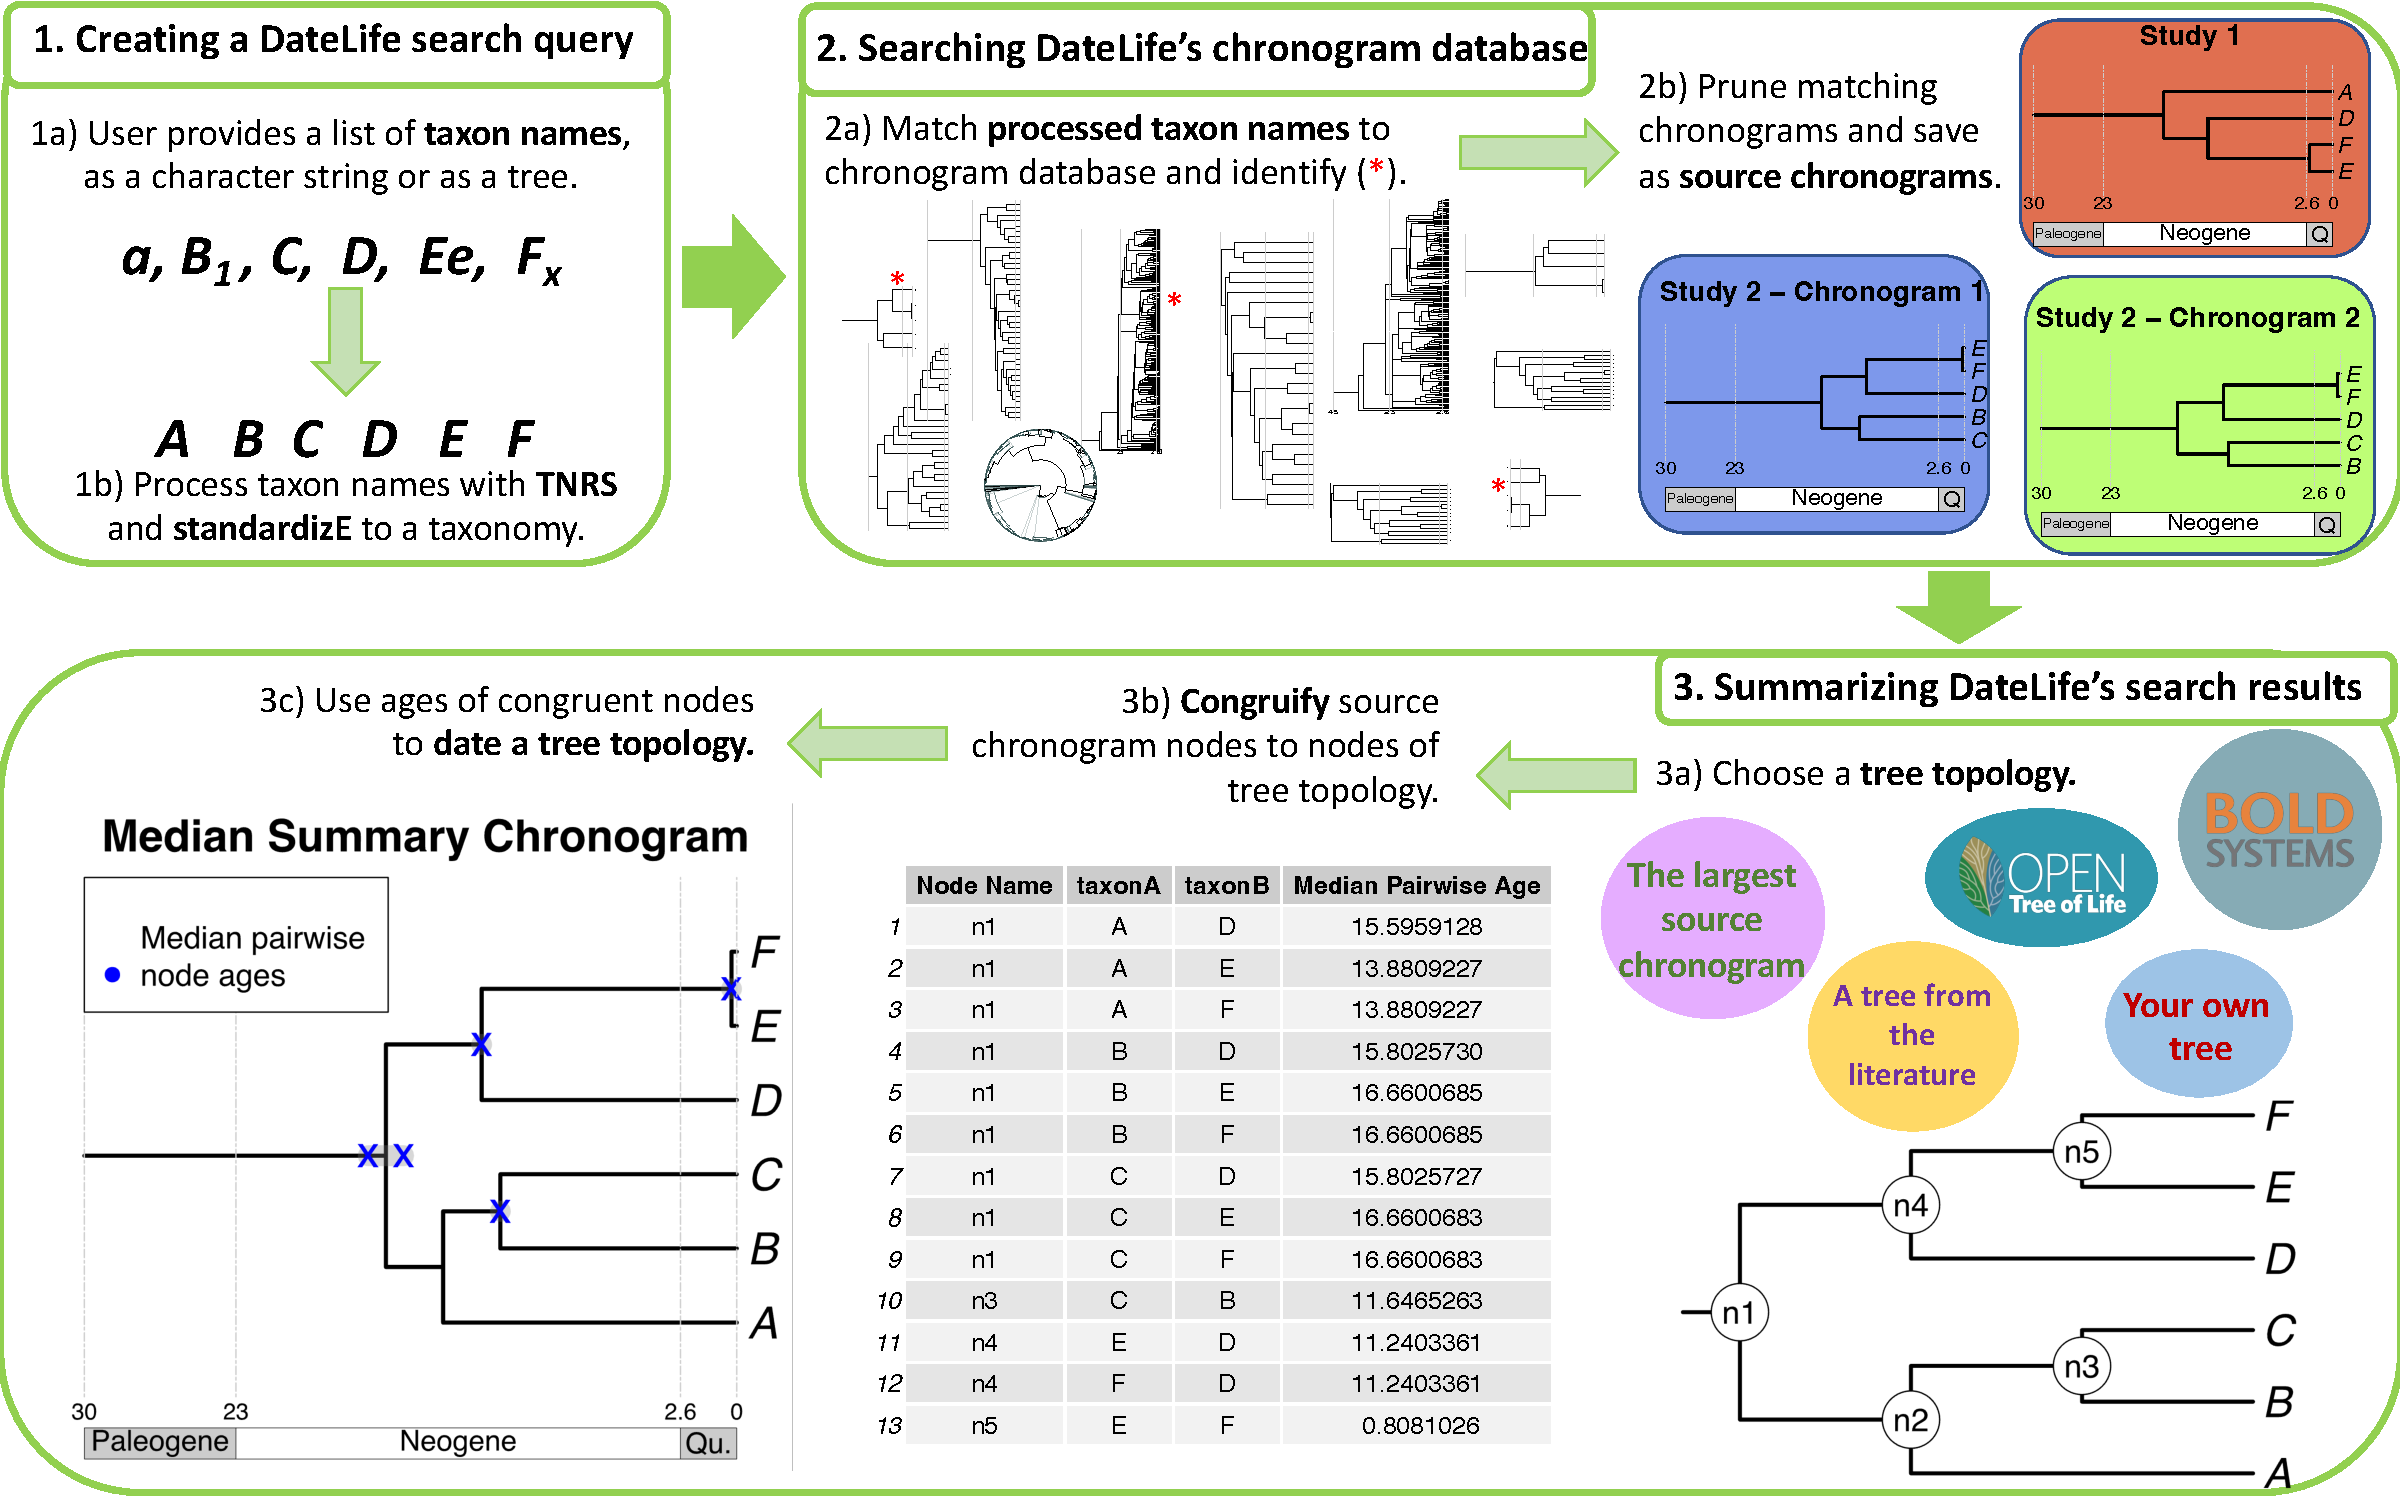
\includegraphics{../figures/figure1/figure1-new.pdf}
\caption{Stylized DateLife workflow. This shows the general worflows and analyses that can be performed with \texttt{datelife}, via the R package or through the website  at \url{http://www.datelife.org/}. Details on the functions involved on each workflow are shown in \texttt{datelife}'s R package vignette.
}
\label{fig:workflow}
\end{figure}
% \begin{center}
% \textsc{Figure \ref{fig:workflow}}
% \end{center}

\begin{figure}[!h]
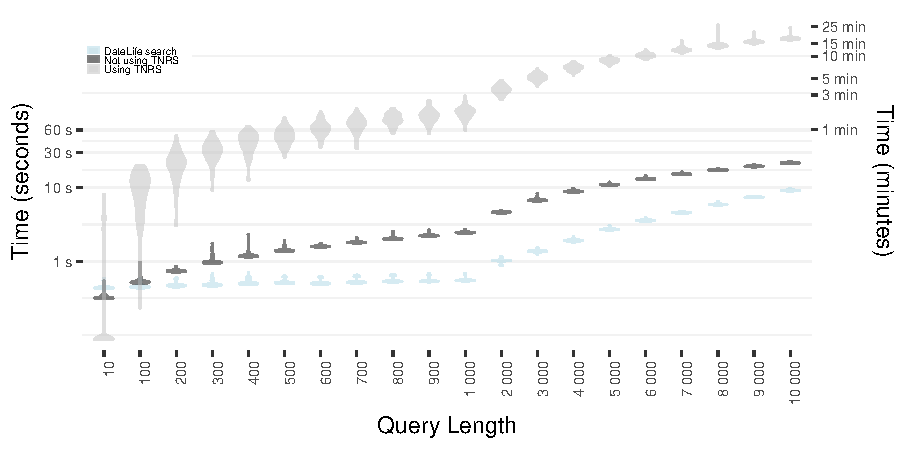
\includegraphics[width=1\linewidth]{../figures/fig_runtime_main.pdf}
\caption{Computation time of query processing and search across \texttt{datelife}'s chronogram database relative to number of input taxon names. We sampled N names from the class Aves for each cohort 100 times and then performed a search with query processing not using the Taxon Names Resoultion Service (TNRS; dark gray), and using TNRS (light gray). We also performed a search using the already processed query for comparison (light blue).}
\label{fig:runtime_main}
\end{figure}
% \begin{center}
% \textsc{Figure \ref{fig:benchmark}}
% \end{center}

\begin{figure}[!h]
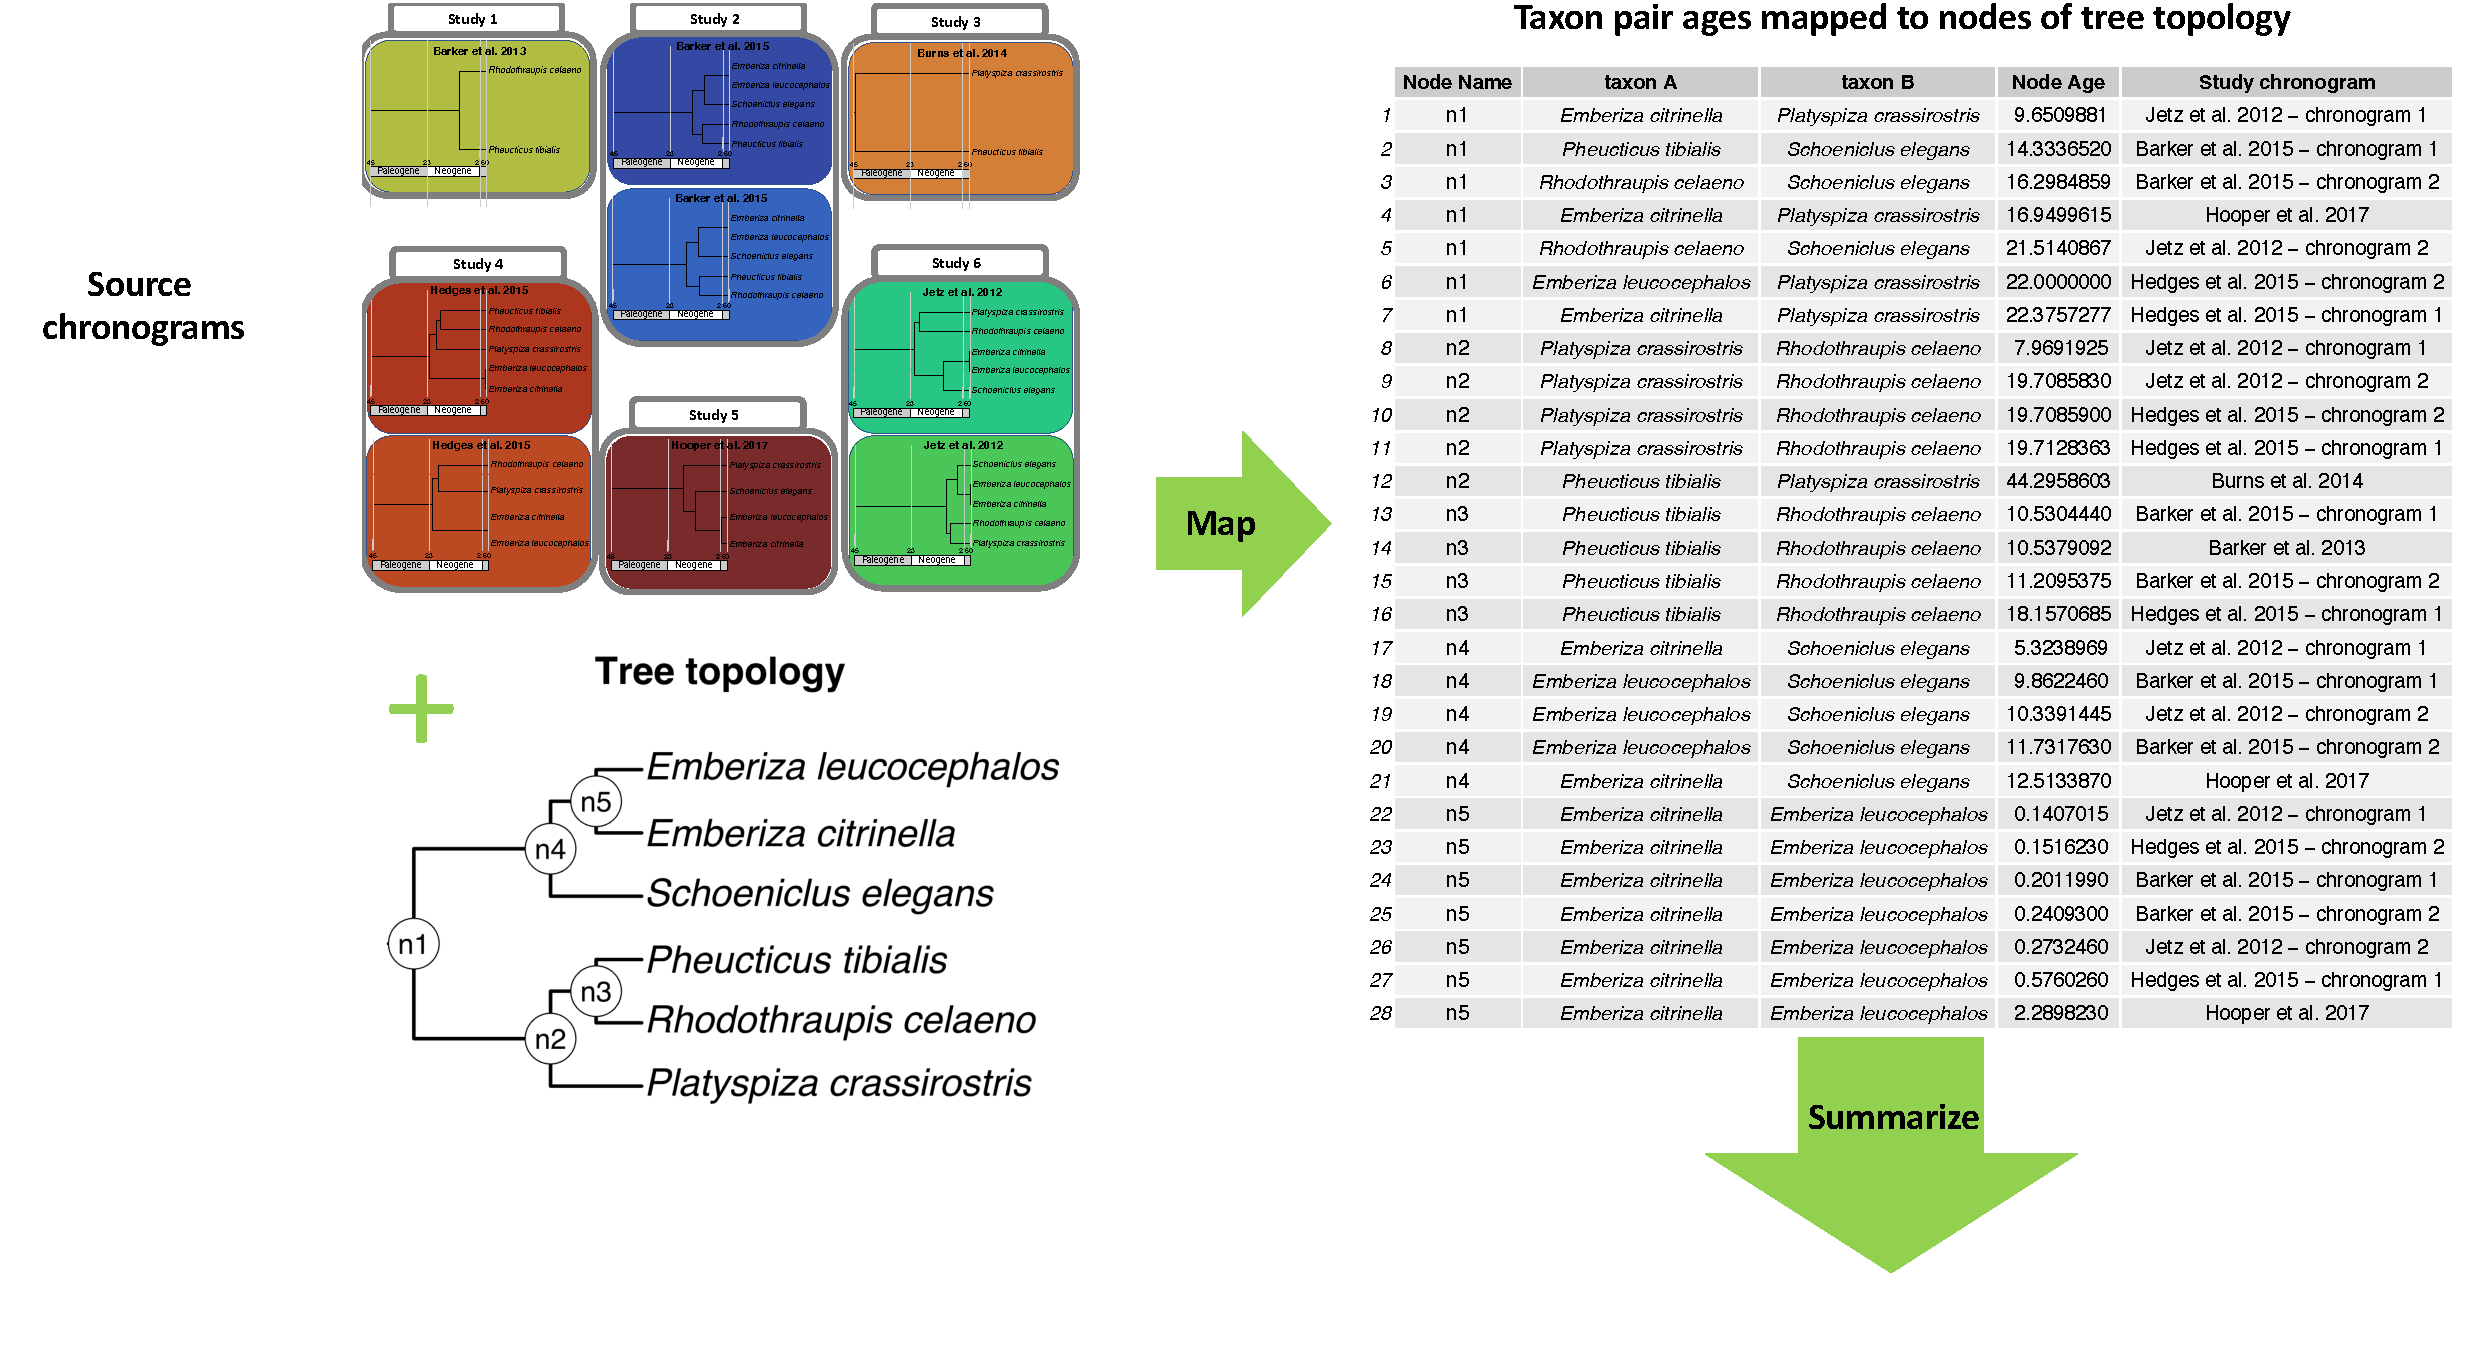
\includegraphics[width=1\linewidth]{../figures/figure2/figure2-1.pdf}
\caption{Age data results of a DateLife search of a small sample of 6 bird species within the Passeriformes. Input names were found across 9 chronograms within 6 independent studies (Barker et al. (\protect\hyperlink{ref-barker2012going}{2012}), Barker et al. (\protect\hyperlink{ref-barker2015new}{2015}), Burns et al. (\protect\hyperlink{ref-burns2014phylogenetics}{2014}), Hedges et al. (\protect\hyperlink{ref-Hedges2015}{2015}), Hooper and Price (\protect\hyperlink{ref-hooper2017chromosomal}{2017}), Jetz et al. (\protect\hyperlink{ref-Jetz2012}{2012}).) This revealed 28 age data points for the queried species names.}
\label{fig:figure2-1}
\end{figure}
% \begin{center}
% \textsc{Figure \ref{fig:figure2-1}}
% \end{center}

\begin{figure}[!h]
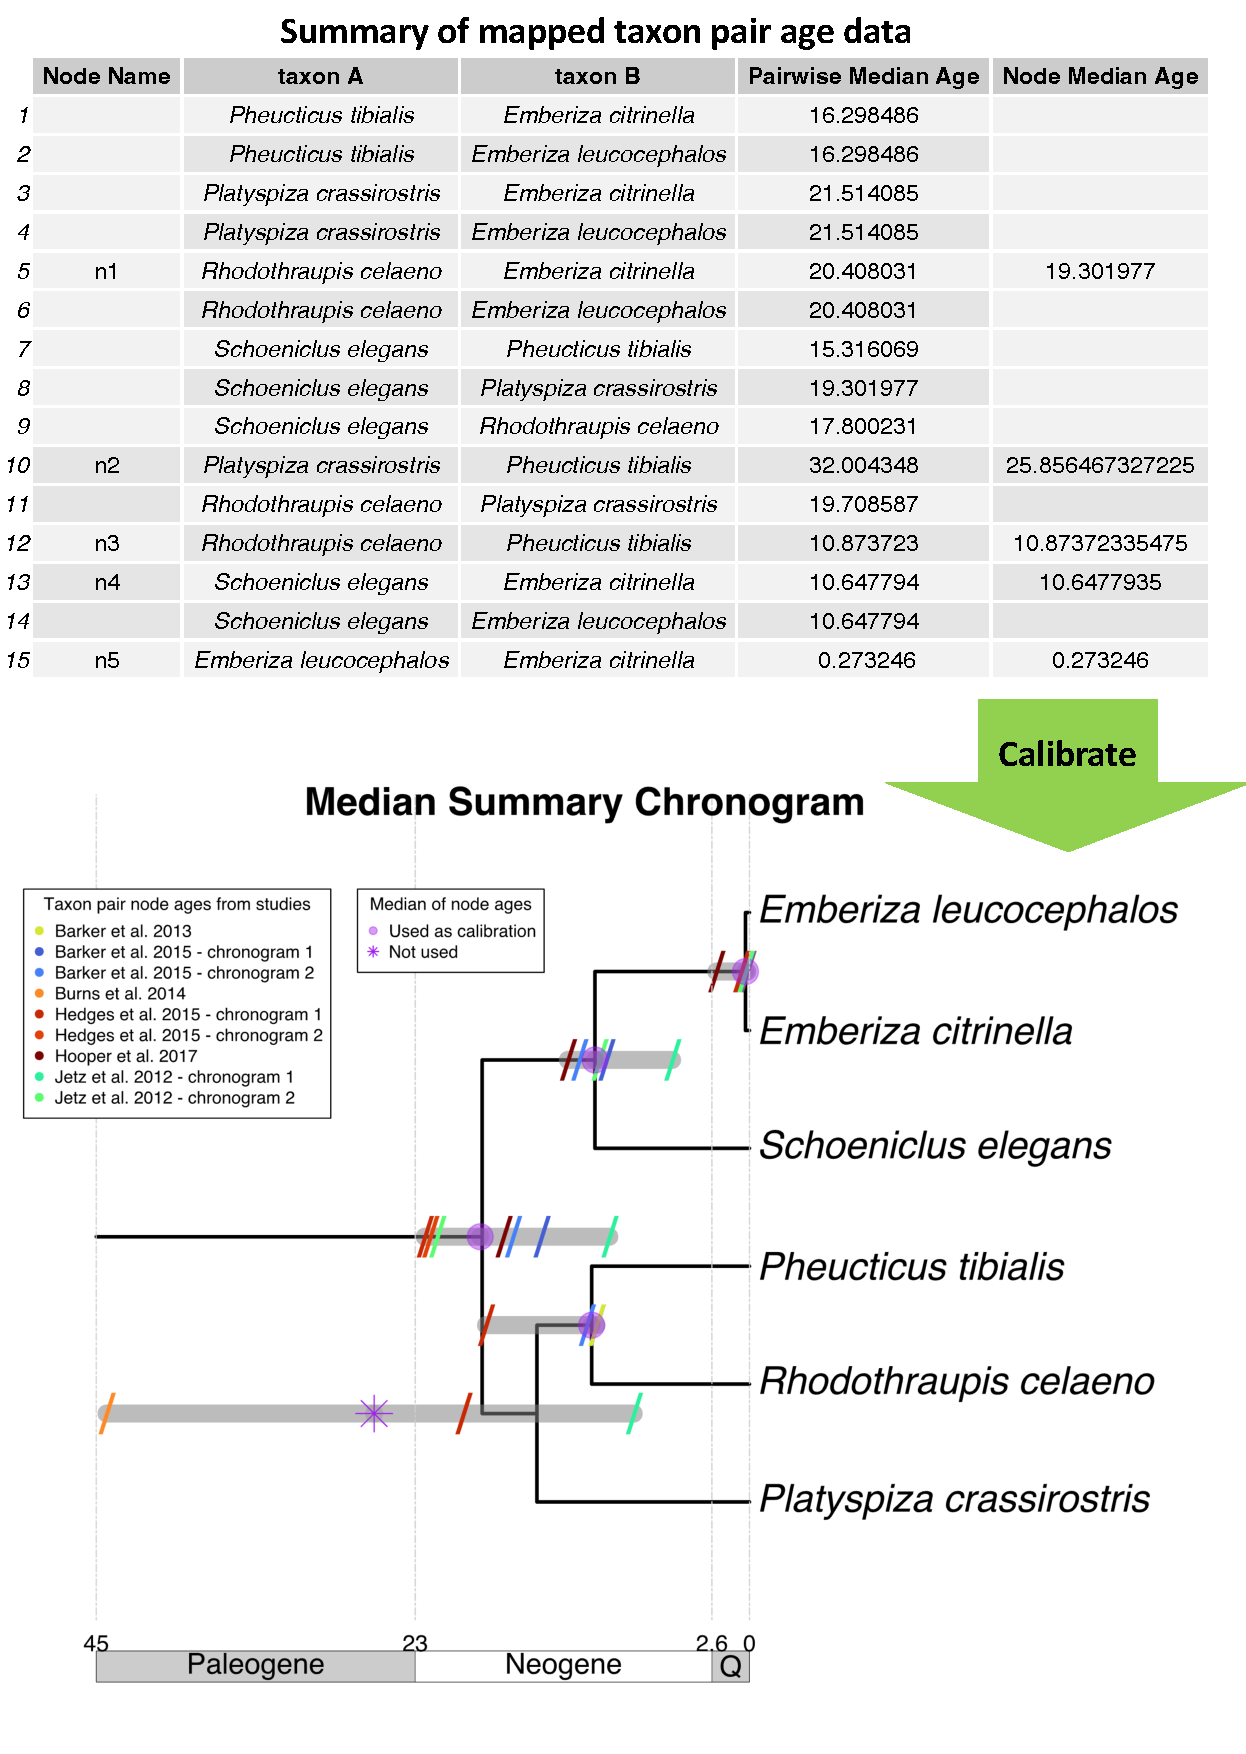
\includegraphics{../figures/figure2/figure2-2.pdf}
\caption{Summarized age data is used as secondary calibrations to date a tree topology as a summary chronogram.}
\label{fig:summaries}
\end{figure}
% \begin{center}
% \textsc{Figure \ref{fig:figure2-2}}
% \end{center}

\begin{figure}[!h]
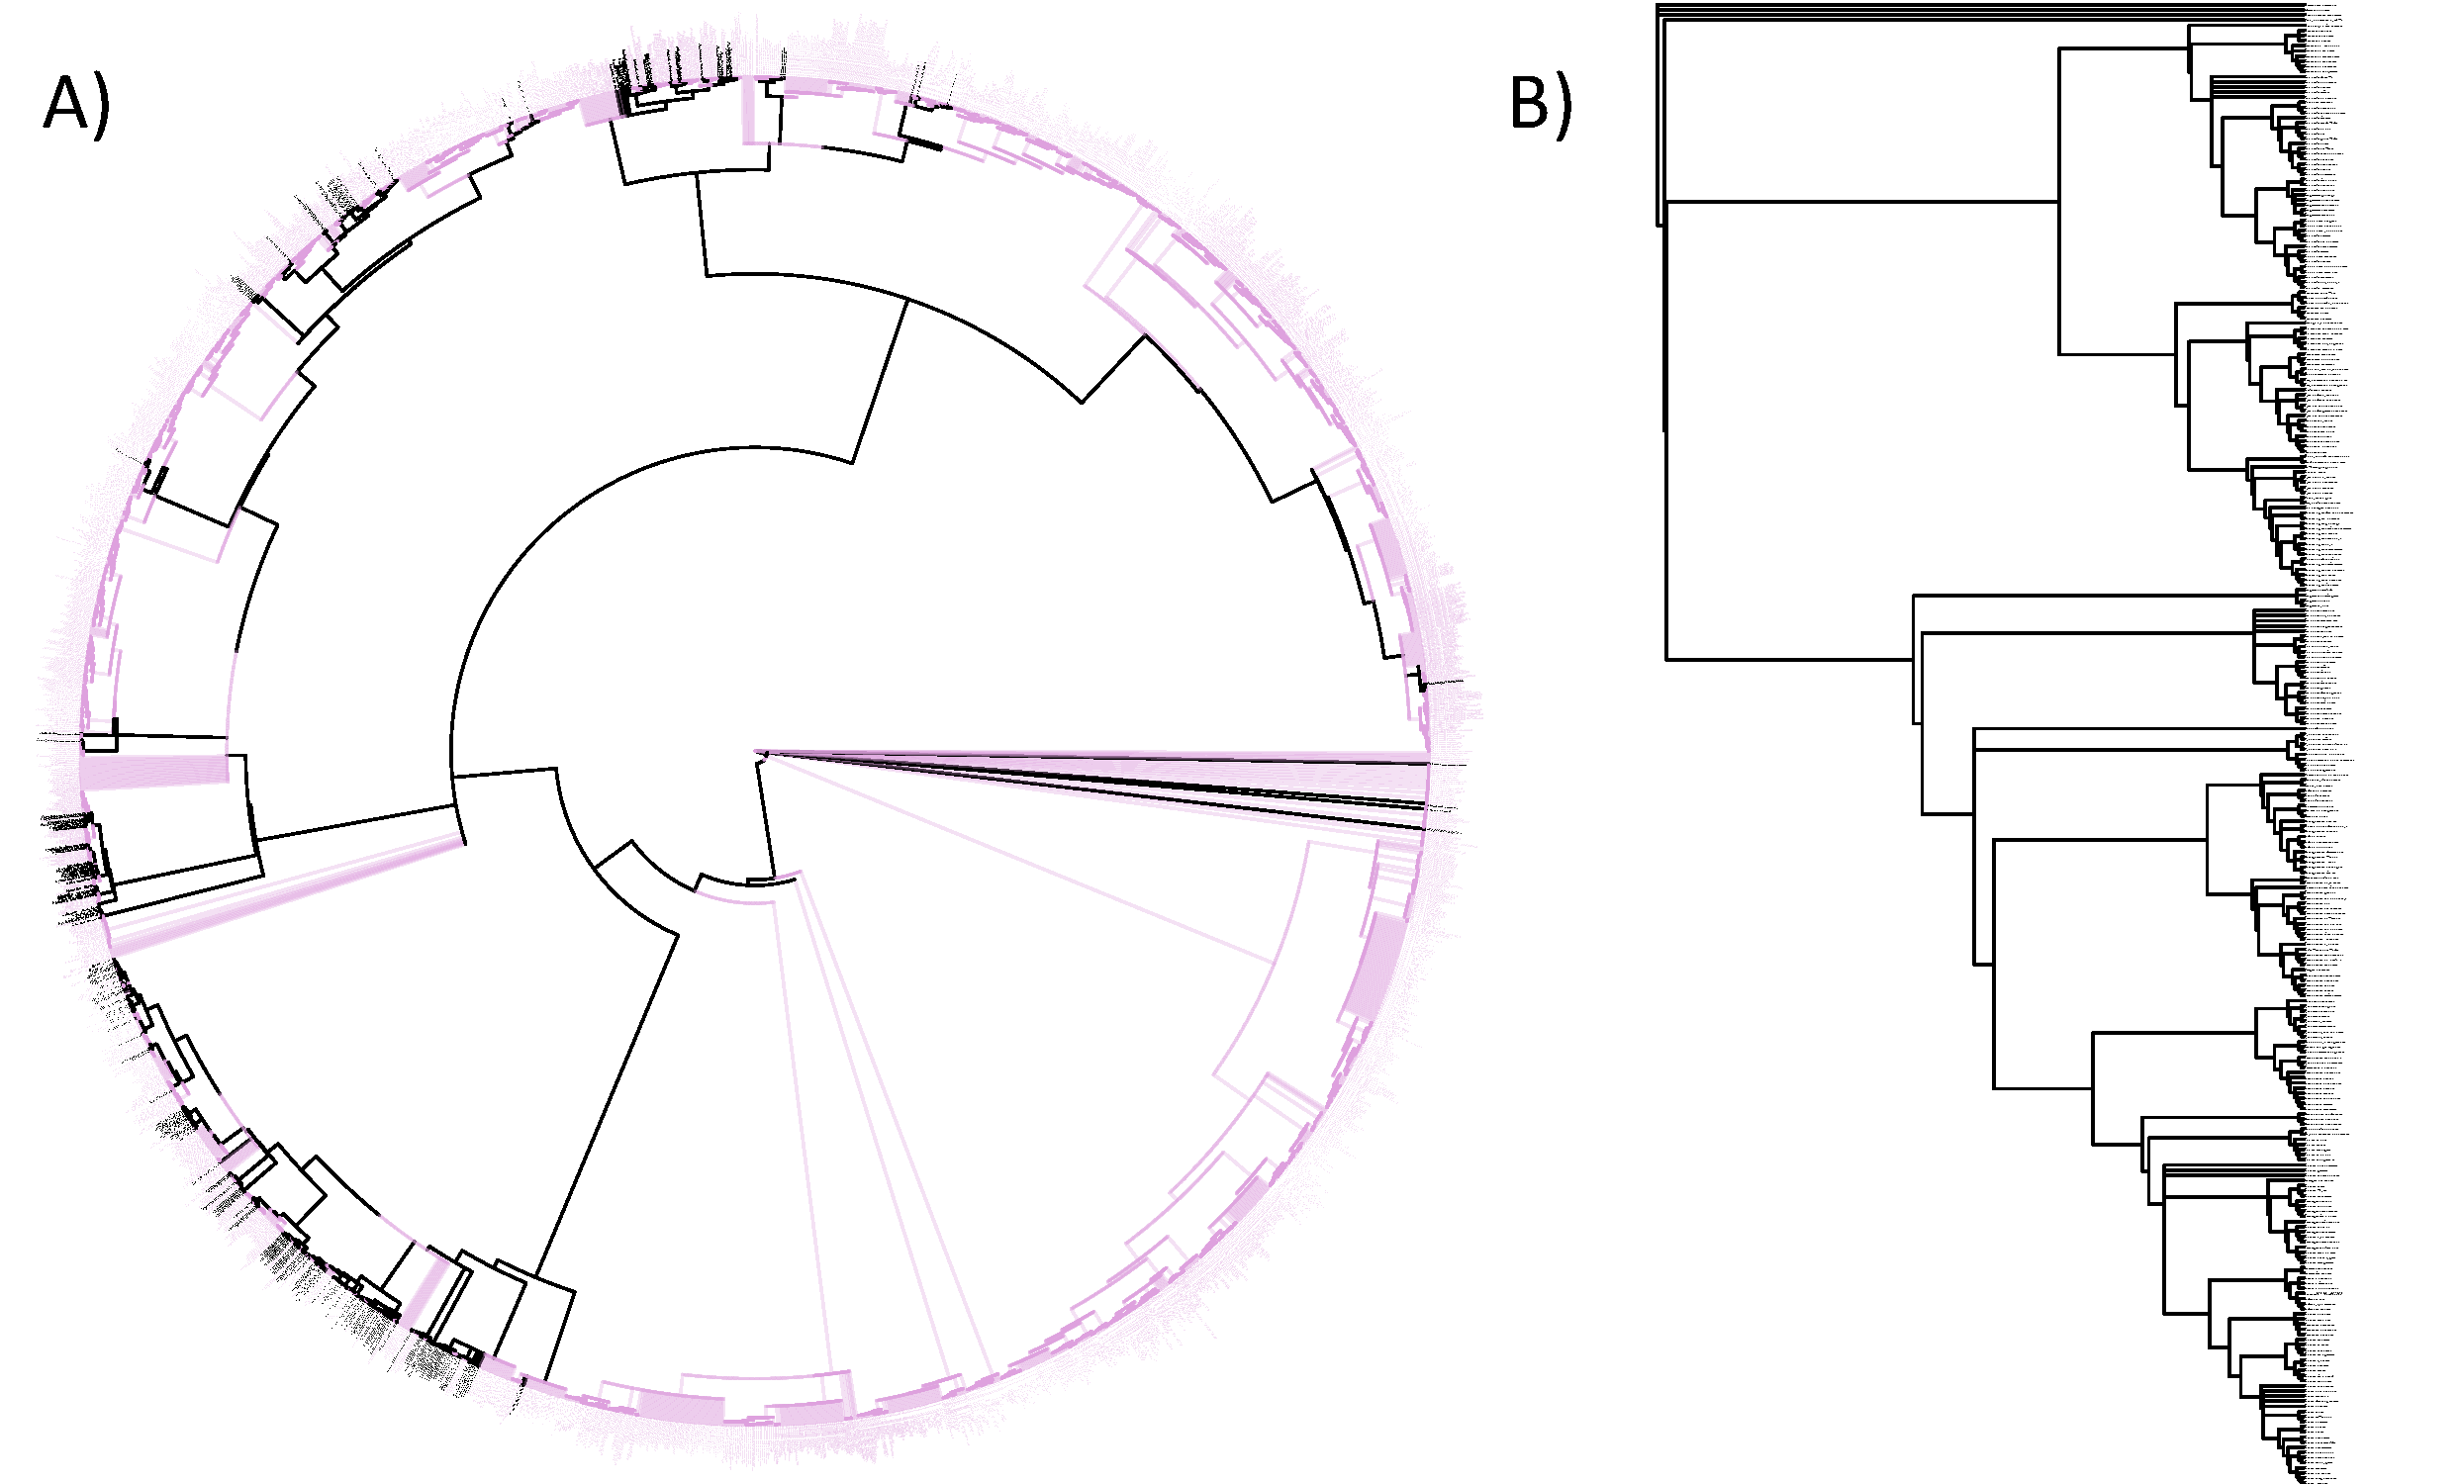
\includegraphics{../figures/fringillidae-topologies/fringillidae-topology.pdf}
\caption{Fringillidae topologies available from OpenTree's synthetic phylogeny. A) Topology encompassing bird species within the Fringillidae within the NCBI taxonomy (black) as well as all species that share the same mrca node in the synthetic tree (purple). B) Paraphyletic topology encompassing bird species within the Fringillidae only. It results from pruning purple branches from topology in A.
Bird species belonging to the family Fringillidae do not form a monophyletic group.
(Alström et al. \protect\hyperlink{ref-}{2014},
Barker, Cibois, Schikler, Feinstein, \& Cracraft \protect\hyperlink{ref-barker2004phylogeny}{2004},
Barker et al. \protect\hyperlink{ref-barker2013going}{2013},
Barker \protect\hyperlink{ref-barker2014mitogenomic}{2014},
Barker et al. \protect\hyperlink{ref-barker2015new}{2015},
Beresford, Barker, Ryan, \& Crowe \protect\hyperlink{ref-beresford2005african}{2005},
Bryson Jr et al. \protect\hyperlink{ref-bryson2014diversification}{2014},
Burleigh, Kimball, \& Braun \protect\hyperlink{ref-burleigh2015building}{2015},
Burns et al. \protect\hyperlink{ref-burns2014phylogenetics}{2014},
Chaves, Hidalgo, \& Klicka \protect\hyperlink{ref-chaves2013biogeography}{2013},
Claramunt \& Cracraft \protect\hyperlink{ref-claramunt2015new}{2015},
Gibb et al. \protect\hyperlink{ref-gibb2015new}{2015},
Hackett et al. \protect\hyperlink{ref-hackett2008phylogenomic}{2008},
Jetz et al. \protect\hyperlink{ref-Jetz2012}{2012},
Johansson, Fjeldså, \& Bowi \protect\hyperlink{ref-johansson2008phylogenetic}{200},
Kimball et al. \protect\hyperlink{ref-kimball2019phylogenomic}{2019},
Klicka et al. \protect\hyperlink{ref-klicka2014comprehensive}{2014},
Lamichhaney et al. \protect\hyperlink{ref-lamichhaney2015evolution}{2015},
Lerner, Meyer, James, Hofreiter, \& Fleischer \protect\hyperlink{ref-lerner2011multilocus}{2011},
Lovette et al. \protect\hyperlink{ref-lovette2010comprehensive}{2010},
Moyle et al. \protect\hyperlink{ref-moyle2016tectonic}{2016},
Ödeen, Håstad, \& Alström \protect\hyperlink{ref-odeen2011evolution}{2011},
Oliveros et al. \protect\hyperlink{ref-oliveros2019earth}{2019},
Päckert et al. \protect\hyperlink{ref-packert2012horizontal}{2012},
Parchman, Benkman, \& Mezquida \protect\hyperlink{ref-parchman2007coevolution}{2007},
Powell et al. \protect\hyperlink{ref-powell2014comprehensive}{2014},
Price et al. \protect\hyperlink{ref-price2014niche}{2014},
Pulgarín-R, Smith, Bryson Jr, Spellman, \& Klicka \protect\hyperlink{ref-pulgarin2013multilocus}{2013},
Selvatti, Gonzaga, \& Moraes Russo \protect\hyperlink{ref-selvatti2015paleogene}{2015},
Tietze, Päckert, Martens, Lehmann, \& Sun \protect\hyperlink{ref-tietze2013complete}{2013},
Treplin et al. \protect\hyperlink{ref-treplin2008molecular}{2008},
Zuccon, Prŷs-Jones, Rasmussen, \& Ericson \protect\hyperlink{ref-zuccon2012phylogenetic}{2012})
}
\label{fig:fringillidae-topologies}
\end{figure}




\begin{figure}[!h]
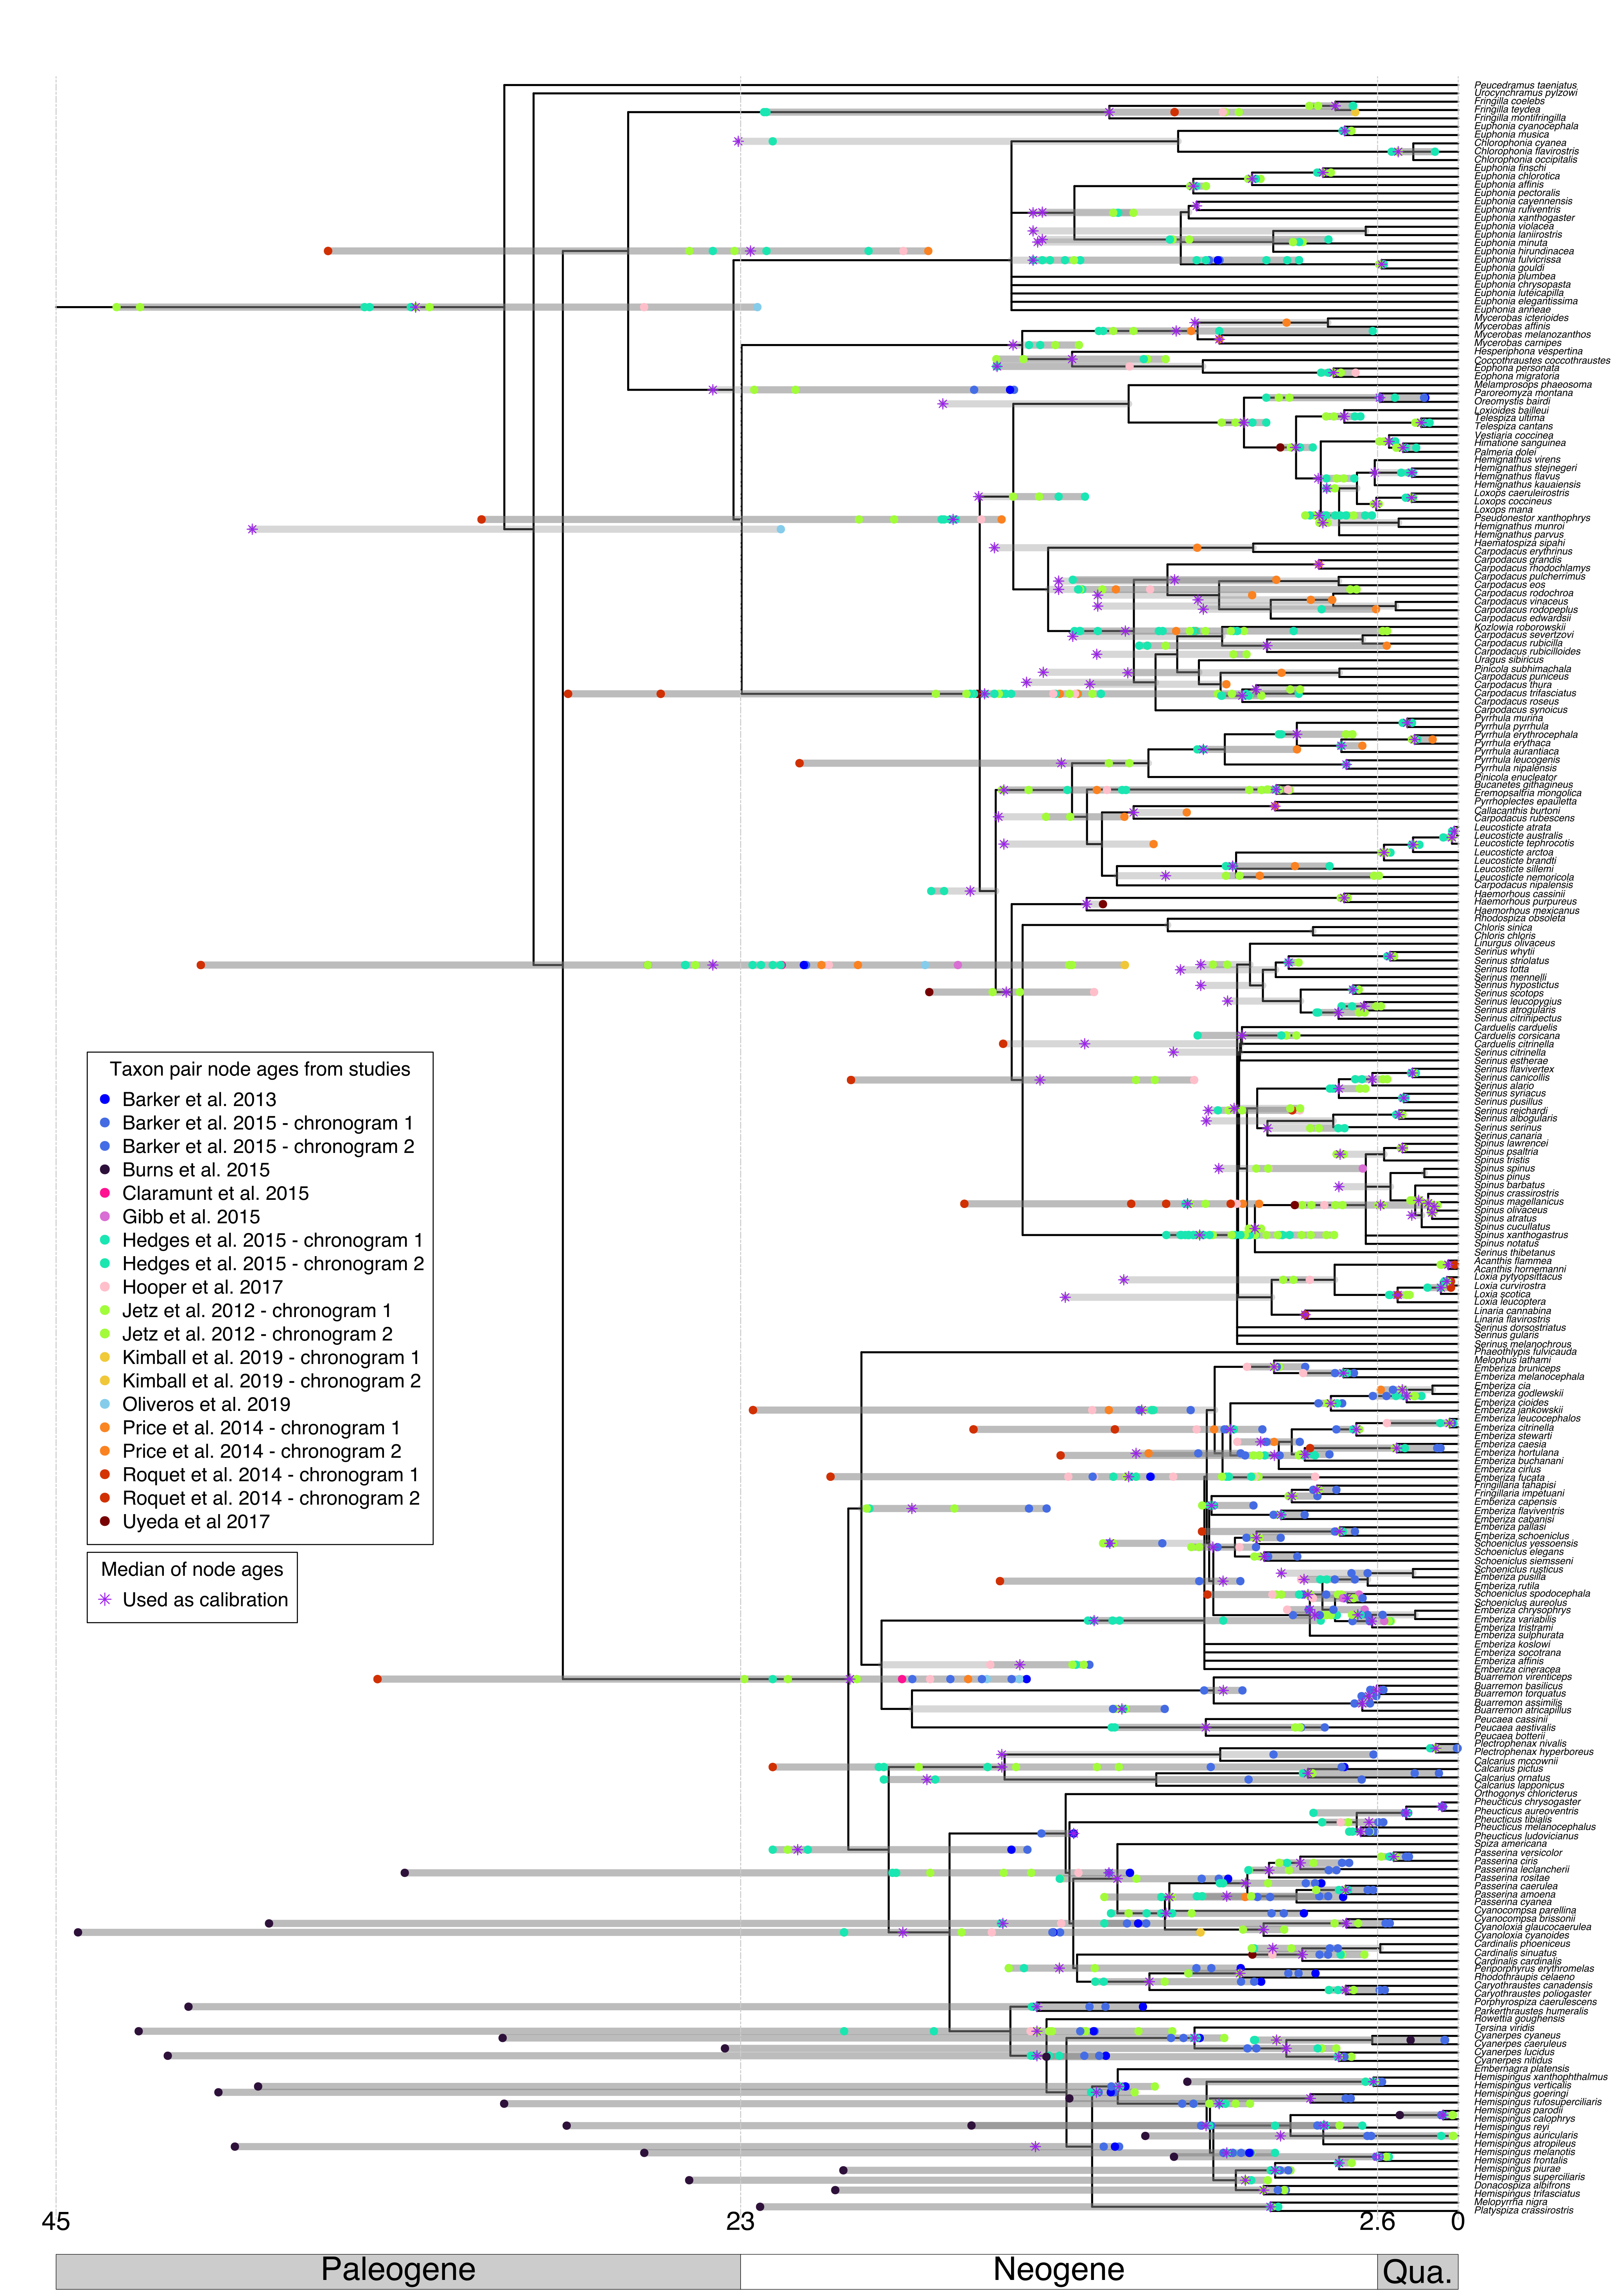
\includegraphics{../figures/figure-fringillidae/median_and_calibration_ages_simple.png}
\caption{Fringillidae median summary chronogram genertaed with DateLife. It has 256 tips and 233 nodes.}
\label{fig:fringillidages}
\end{figure}
% \begin{center}
% \textsc{Figure \ref{fig:fringillidages}}
% \end{center}


% \end{linenumbers}

% in this file I leave the figure captions outside\ caption{} because I want them
% to be formatted in the same way as the general text (double spaced and linenumbered)
\captionsetup[figure]{labelfont={sc},labelformat={default},labelsep=period,name={Figure}}

\begin{figure}[!h]
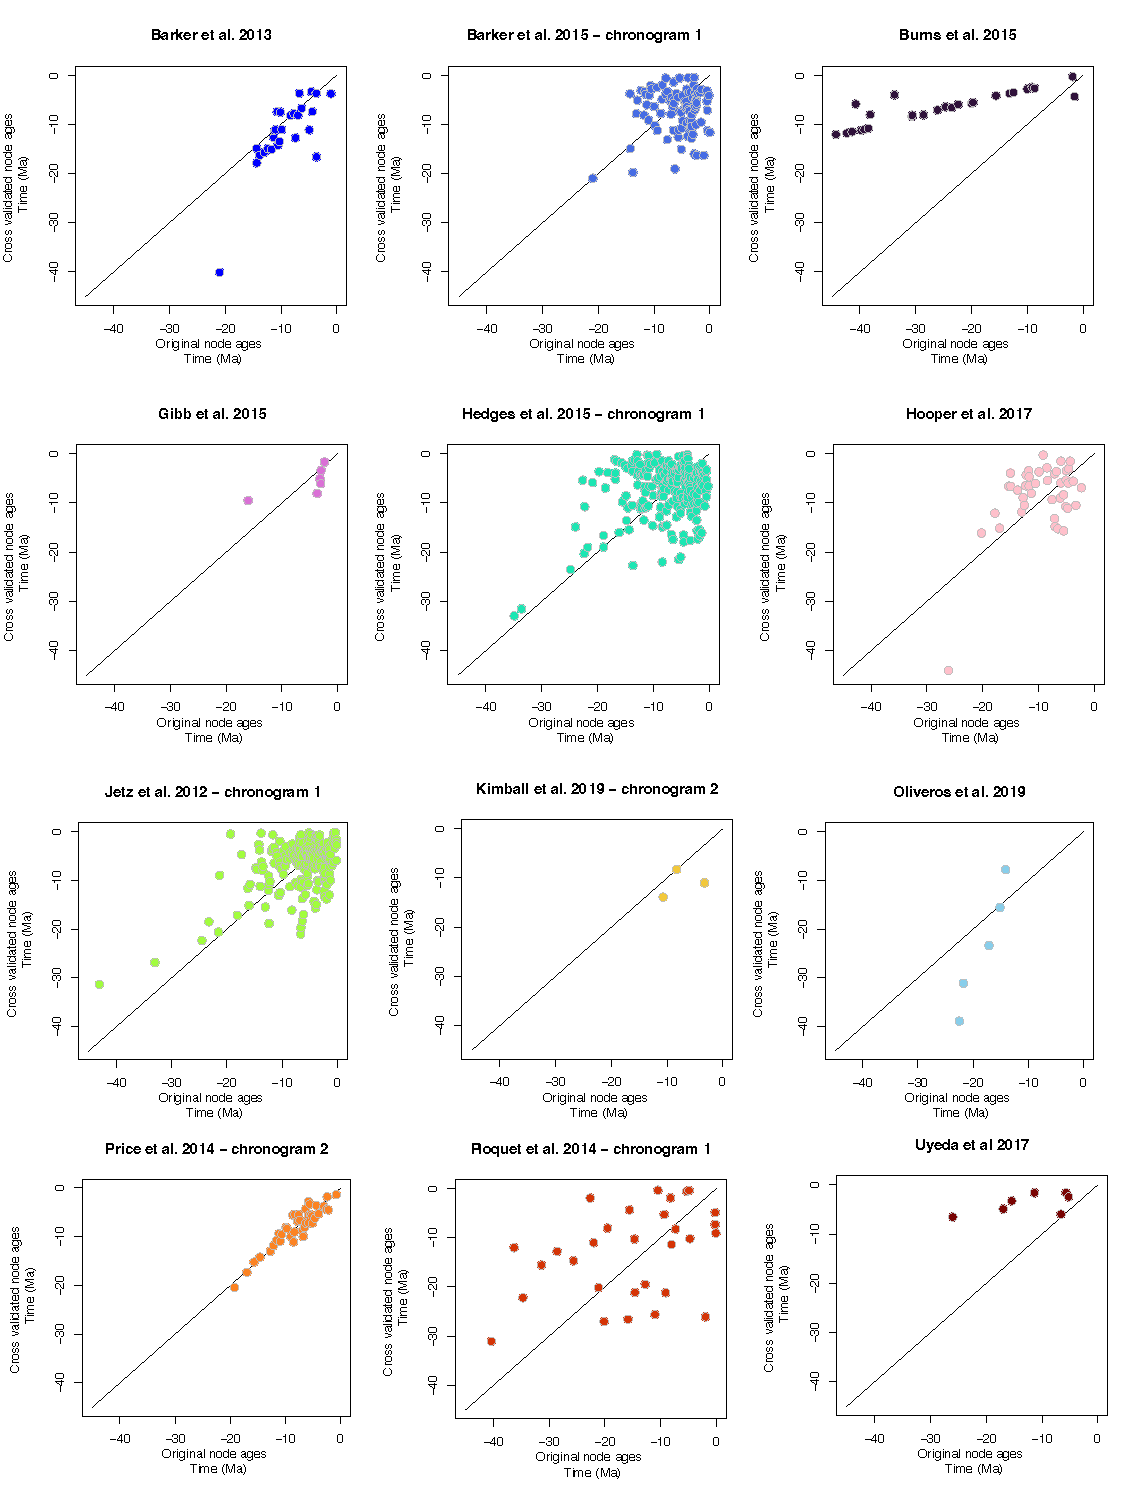
\includegraphics{../figures/figure-cross-validation/fig-cross-validation-xy-plots.pdf}
\caption{Results from cross validation analysis.}
\label{fig:cvXY}
\end{figure}

\begin{figure}[!h]
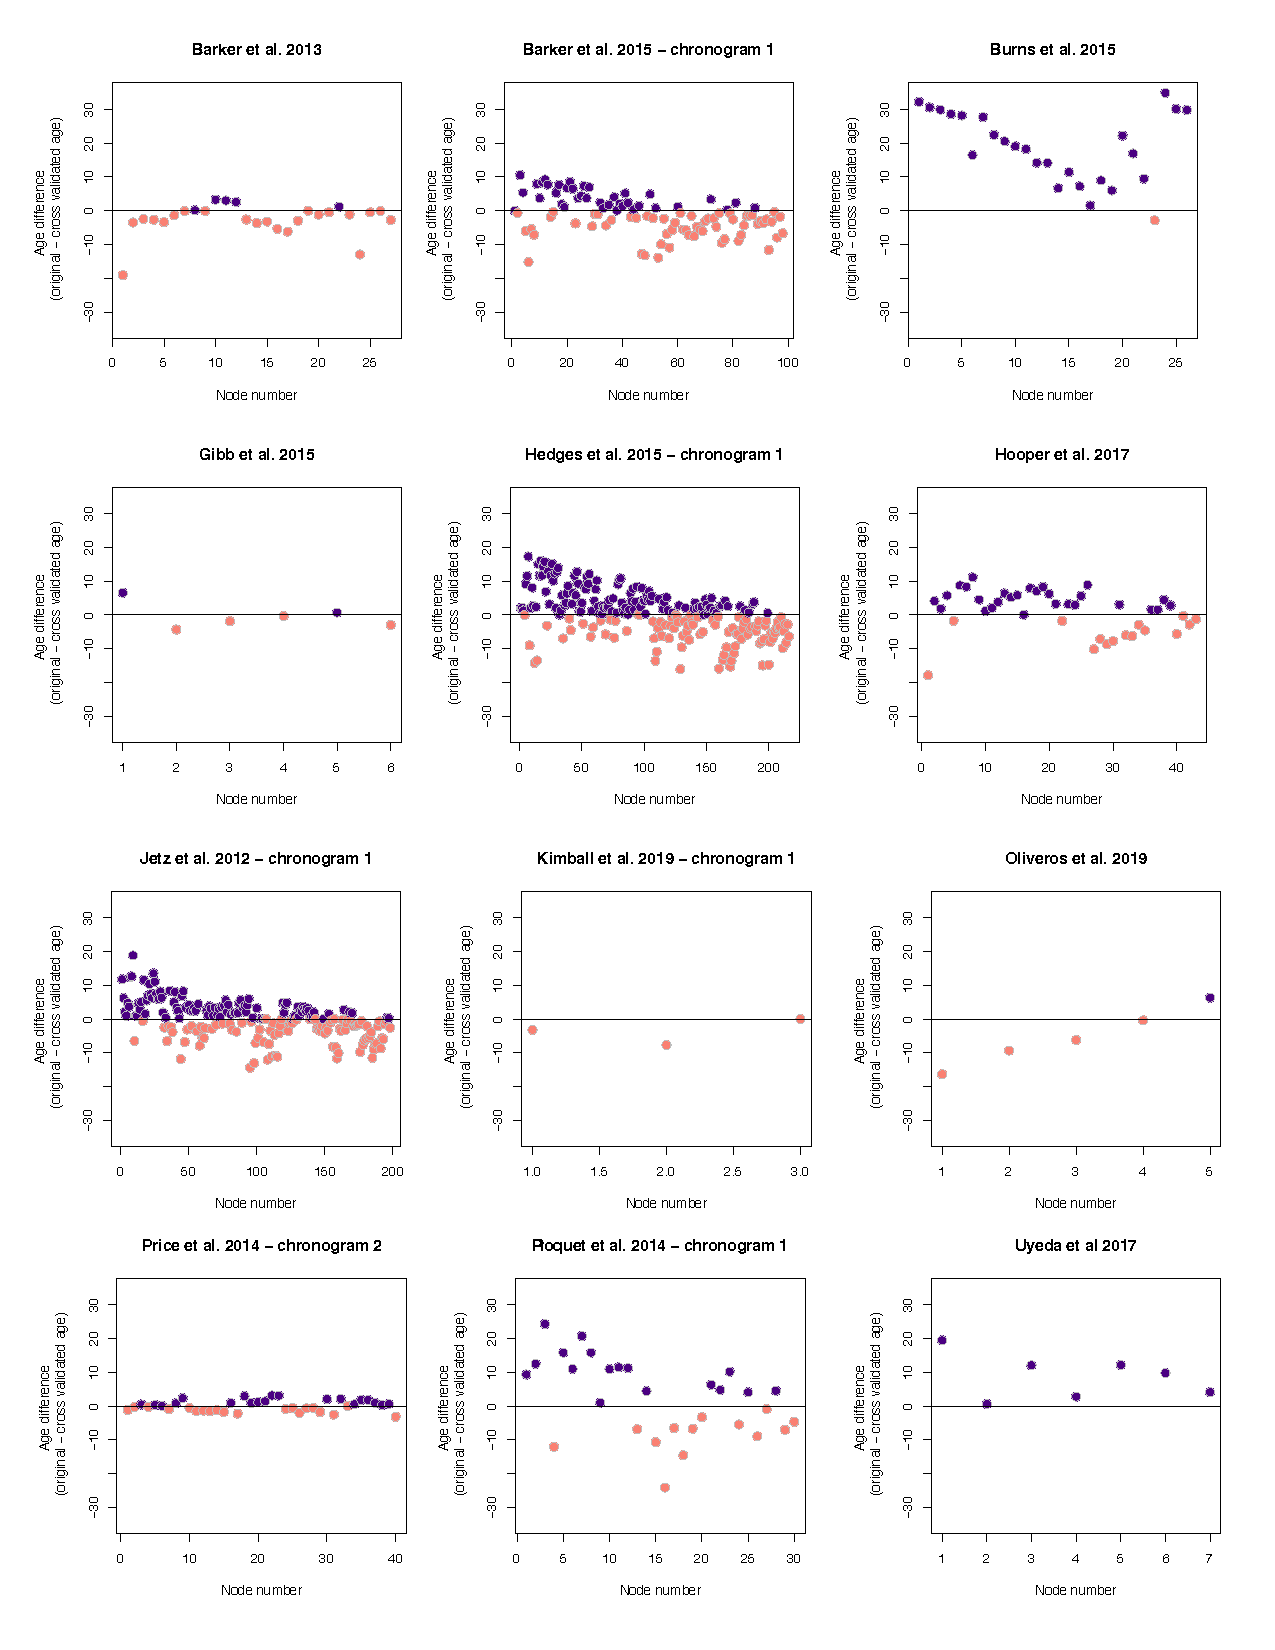
\includegraphics{../figures/figure-cross-validation/fig-cross-validation-xy-plots-diffs.pdf}
\caption{Results from cross validation analysis.}
\label{fig:cvXYdiffs}
\end{figure}

\begin{figure}[!h]
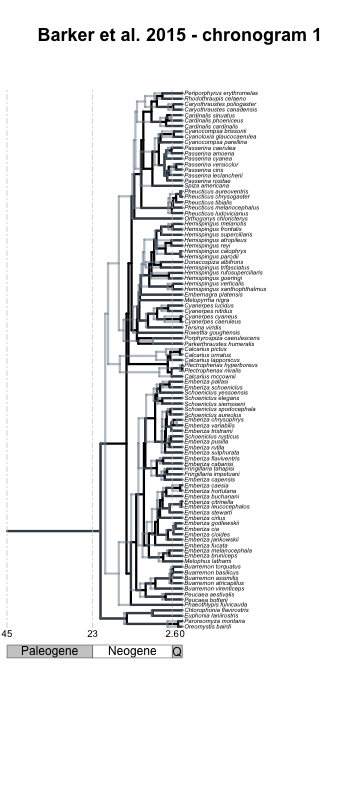
\includegraphics{../figures/figure-cross-validation/cross_validation_2.png}
\caption{Cross validation of second source chronogram. The chronogram shown in black corresponds to the dates published in the original study. The gray chronogram corresponds to the same tree topology dated with BLADJ using node ages from all other source chronograms as secondary calibrations.}
\label{fig:cv2}
\end{figure}

\begin{figure}[!h]
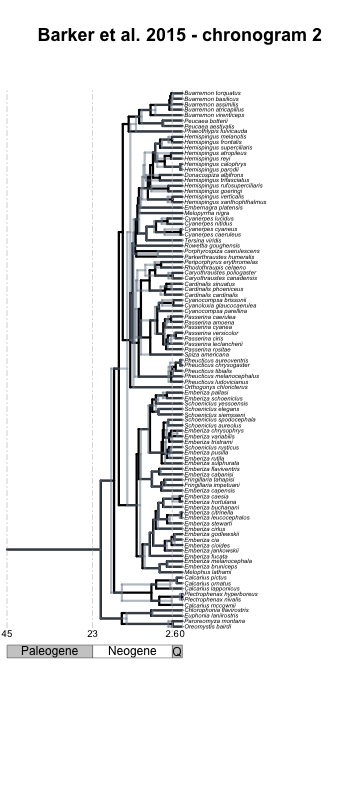
\includegraphics{../figures/figure-cross-validation/cross_validation_3.png}
\caption{Cross validation of third source chronogram. The chronogram shown in black corresponds to the dates published in the original study. The gray chronogram corresponds to the same tree topology dated with BLADJ using node ages from all other source chronograms as secondary calibrations.}
\label{fig:cv3}
\end{figure}

\begin{figure}[!h]
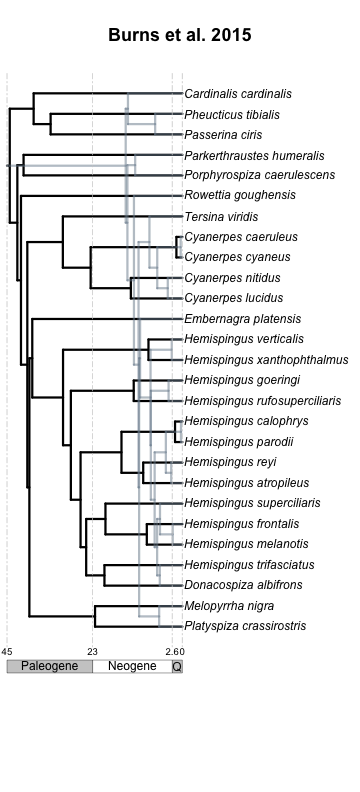
\includegraphics{../figures/figure-cross-validation/cross_validation_4.png}
\caption{Cross validation of fourth source chronogram. The chronogram shown in black corresponds to the dates published in the original study. The gray chronogram corresponds to the same tree topology dated with BLADJ using node ages from all other source chronograms as secondary calibrations.}
\label{fig:cv4}
\end{figure}

\begin{figure}[!h]
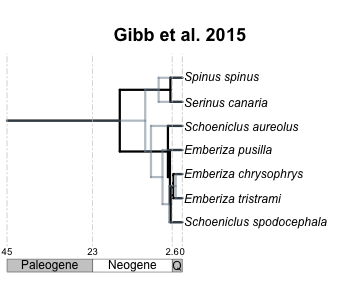
\includegraphics{../figures/figure-cross-validation/cross_validation_6.png}
\caption{Cross validation of sixth source chronogram. The chronogram shown in black corresponds to the dates published in the original study. The gray chronogram corresponds to the same tree topology dated with BLADJ using node ages from all other source chronograms as secondary calibrations.}
\label{fig:cv6}
\end{figure}

\begin{figure}[!h]
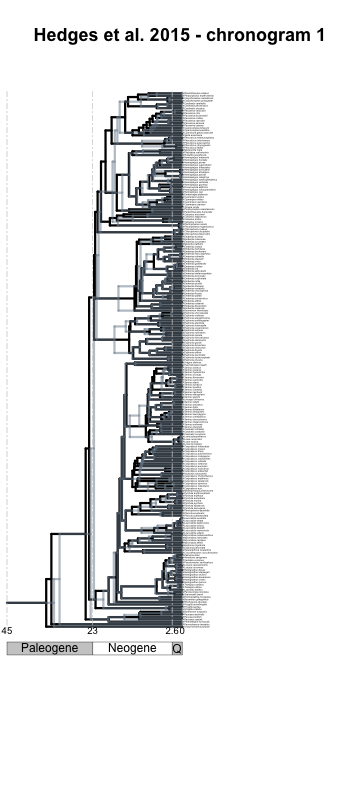
\includegraphics{../figures/figure-cross-validation/cross_validation_7.png}
\caption{Cross validation of seventh source chronogram. The chronogram shown in black corresponds to the dates published in the original study. The gray chronogram corresponds to the same tree topology dated with BLADJ using node ages from all other source chronograms as secondary calibrations.}
\label{fig:cv7}
\end{figure}

\begin{figure}[!h]
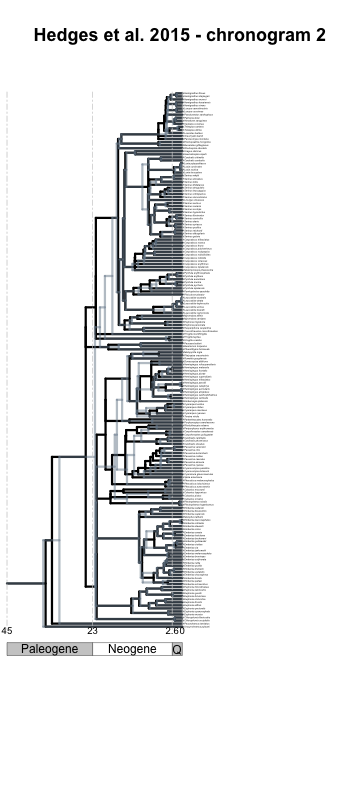
\includegraphics{../figures/figure-cross-validation/cross_validation_8.png}
\caption{Cross validation of eight source chronogram. The chronogram shown in black corresponds to the dates published in the original study. The gray chronogram corresponds to the same tree topology dated with BLADJ using node ages from all other source chronograms as secondary calibrations.}
\label{fig:cv8}
\end{figure}

\begin{figure}[!h]
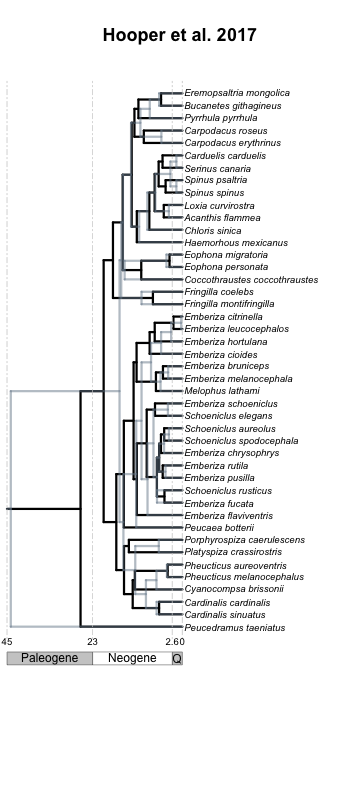
\includegraphics{../figures/figure-cross-validation/cross_validation_9.png}
\caption{Cross validation of ninth source chronogram. The chronogram shown in black corresponds to the dates published in the original study. The gray chronogram corresponds to the same tree topology dated with BLADJ using node ages from all other source chronograms as secondary calibrations.}
\label{fig:cv9}
\end{figure}

\begin{figure}[!h]
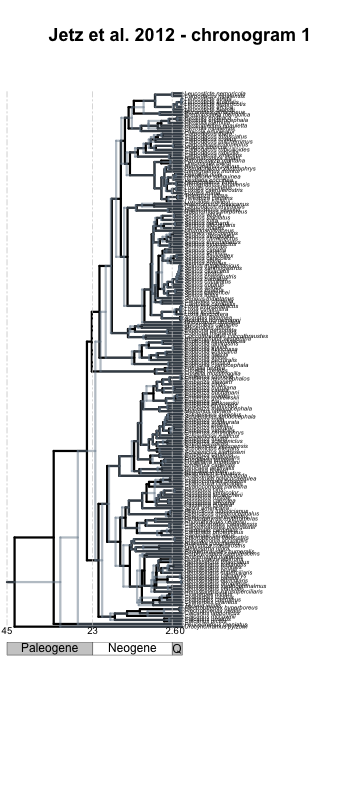
\includegraphics{../figures/figure-cross-validation/cross_validation_10.png}
\caption{Cross validation of tenth source chronogram. The chronogram shown in black corresponds to the dates published in the original study. The gray chronogram corresponds to the same tree topology dated with BLADJ using node ages from all other source chronograms as secondary calibrations.}
\label{fig:cv10}
\end{figure}

\end{document}
